\documentclass[conference,onecolumn]{IEEEtran}
\usepackage{hyperref}
\usepackage[utf8]{inputenc}
\usepackage[french]{babel}
\usepackage{amsmath,amssymb,amsfonts}
\usepackage{mathtools}
\usepackage{algorithmic}
\usepackage{graphicx}
\usepackage{textcomp}
\usepackage{xcolor}
\usepackage{float}
\usepackage{lipsum, babel}
\usepackage[T1]{fontenc}
\usepackage{biblatex}
\usepackage{ragged2e}
\usepackage{geometry}
\geometry{
   hmargin=3cm,
   vmargin=2cm,
   includeheadfoot
}

\pagestyle{plain}

% Inicio del documento
\begin{document}

\title{Atténuation du bruit dans des signaux audios a travers l’implémentation de méthodes classiques et une méthode hybride\\
}

\author{\IEEEauthorblockN{1\textsuperscript{st} José Miguel Galindo Barco}
\IEEEauthorblockA{\textit{Ecole d’ingénieurs}\\
\textit{Génie de systèmes} \\
\textit{Université EAFIT}\\
\href{mailto:jmgalindob@eafit.edu.co}{jmgalindob@eafit.edu.co}
}
\and
\IEEEauthorblockN{2\textsuperscript{nd} Juan José Tamayo Acevedo}
\IEEEauthorblockA{\textit{Ecole de sciences}\\
\textit{Génie mathématique} \\
\textit{Université EAFIT}\\
\href{mailto:jjtamayoa@eafit.edu.co}{jjtamayoa@eafit.edu.co}
}
\and
\IEEEauthorblockN{3\textsuperscript{rd} Salomón Cardeño Luján}
\IEEEauthorblockA{\textit{Ecole de sciences}\\
\textit{Génie mathématique} \\
\textit{Université EAFIT}\\
\href{mailto:scardenol@eafit.edu.co}{scardenol@eafit.edu.co}
}
}

\maketitle

\begin{abstract}
L’atténuation du bruit est un domaine d’étude actif dans des milieux comme le traitement digital et analogique des signaux. Dans ce domaine il existe une grande variété d’algorithmes et/ou méthodes classiques et modernes qui sont utilisé dans ce but. Dans ce travail de recherche, nous réaliserons une étude théorique du filtre analogique passe-bas avec une approximation de Butterworth, le filtre de Weiner et la méthode dite hybride de DSP/Deep Learning RNNbruit. Puis nous développerons une analyse de ces trois méthodes où nous comparerons les résultats de signaux lorsque nous filtrons un signal propre, un signal avec addition de bruit blanc, un signal avec addition de bruit rosa et un signal avec addition de bruit rouge. Les enregistrement audios résultant de chaque méthode filtrage seront comparer qualitativement et quantitativement, d’où la nécessité de tenir en compte la perception auditive du récepteur. Finalement, nous proposerons des modifications sur la mise en œuvre ou implémentation de ces méthodes en considérant le contexte et le bon fonctionnement dans ce dernier. 
\end{abstract}

\section{Introduction}


\section{Concepts fondamentaux}

\begin{itemize} % Lista
    \item[] \textbf{Signal}: un signal est la representation physique de l'information, qu'il convoit de sa source a sa destination.

    \item[] \textbf{Bruit}: Un bruit correspond a tout phénomène gênant la transmission ou l'interpretation d'un signal

    \item[] \textbf{Traitement du signal}: Le traitement du signal est une discipline qui étudie des méthodes de traitement, d’analyse et d’interprétation des signaux. Pour cela, dans ce domaine on utilise des méthodes tels que le contrôle, le filtrage, la compression et la transmission de données, la réduction du bruit, la déconvolution, la prédiction, l'identification, la classification.  

    \item[] \textbf{Filtrage}: On appelle "filtrage" toute application qui, à un signal $f_e(t)$, dit "signal d'entrée", associe un signal $f_s(t)$, dit "signal de sortie", tel que le module du spectre de $f_s(t)$ soit inférieur ou égal au module du spectre de $f_s(t)$, pour w réel quelconque. 
\end{itemize}

\subsection{Signal sonore et note audio}
Le son ou signal sonore est une perturbation mécanique d’un état d’équilibre, qui se propage à travers d’un milieu solide élastique. Il est possible de le définir subjectivement comme ceux qui est perçu par l’ouïe, mais cela reviendra à restreindre la définition même d’un signal. De même, la lumière est perçue par la vue mais il existe certaines longueurs d’ondes lumineuse qui ne sont pas perçu par l’œil humain. Il existe donc des domaines de fréquences des signaux sonores qui ne sont pas perçu par l’ouïe humain. 

Dans un premier temps, en s’appuyant sur le point de vue physique, les ondes sonores se propage à travers l’air ou autres milieux (solides et élastiques) sous forme de longueur d’ondes, où la vibration mécanique qui décrit l’onde se propage dans la même direction que la propagation de celle-ci. L’air peut être compris comme un milieu élastique sur lequel les particules, ou tout simplement les couches d’air, ont un comportement semblable à un ressort, c’est-à-dire qu’elles “se poussent” et “s’attirent” les unes avec les autres. 

Plus clairement, une onde sonore est une variation periodique ou sinusoidale de la pression d’un milieu pendant un temps precis dans un endroit precis. 

Dans la figure ci-dessous, dans un premier temps nous pouvons voir l’air dans son equilibre (figure xA), le variations dans l’air lorsqu’une onde sonore pure se deplace dans ce milieux (figure xB) et l’allure de  l’onde qui se déplace dans l’air.

% Imagen
\begin{figure}[H]
 \centering
    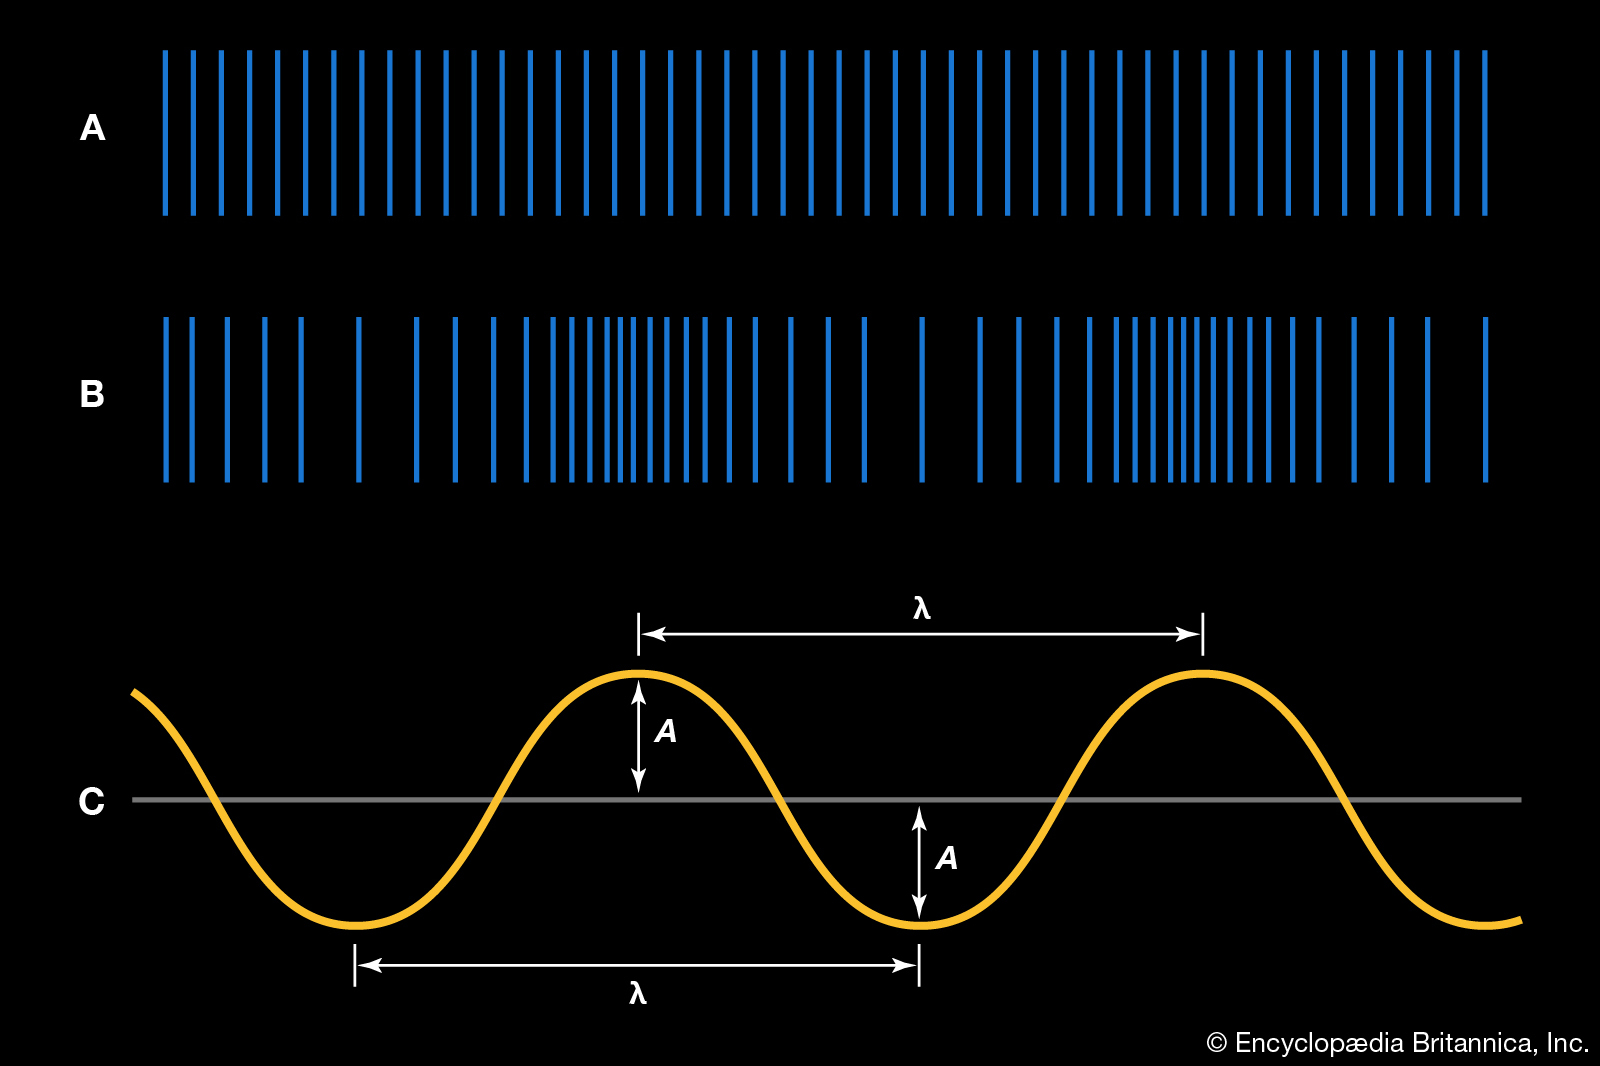
\includegraphics[scale=0.2]{img1.jpg}
    \caption{Représentations graphiques d’une onde sonore. (A) L’air à l’équilibre, avec l’absence de l’onde sonore. (B) compressions et réfractions qui constituent l’onde sonore. (C) Représentation graphique de l’onde sonore avec son amplitude A et sa longueur d’onde $\lambda$.}
\end{figure}

\subsection{Caractéristiques physique et description mathématique d’un signal sonore }

Il est important de remarque que dans figure précédente, plus précisément dans la partie C de cette figure, s’agit d’une autre représentation du signal sonore illustré dans la partie B. En effet, dans cette partie nous pouvons voire une courbe sinusoïdale, cette courbe représente la variation de la pression du signal sonore, celui-ci se répète de façon périodique. La distance entre 2 pics de la courbe est nommée longueur d’onde et se représente par la lettre $\lambda$. 

Lorsqu’un signal sonore ou onde sonore se déplace dans l’air, la longueur d’onde prend un certain temps pour aller d’un point $A$ à un point $B$ de l’espace, cette durée de temps est appelée période et note T. 

De plus, pendant un intervalle de temps équivalent à une seconde, un certain nombre de longueurs d’onde passe d’un point A à un point de l’espace. Ce phénomène est connu comme fréquence du signal. Dans d’autres mots, la fréquence est le nombre de périodes par unité de temps ce qui correspond à l’inverse de la période : $f=1/T$ ou f est la fréquence en Hertz ($Hz$ ou $s^-1$) et $T$ la période en seconde ($s$). 

Il est important de remarquer que les signaux sonores qui ont de hautes fréquences, ont des périodes courtes, alors que les signaux sonores qui ont des bases fréquences, ont de longs périodes. De plus, l’intervalle de fréquences que l’être humain peut percevoir se trouve entre les $20Hz$ et les $20 kHz$. Il existe une propriété physique qui permet de classifier les signaux sonores en fonction de la perception physiologique des êtres humains, cette propriété est connue comme le ton. En plus, les signaux ont une vitesse de déplacement, celle-ci est connue comme vitesse de l’onde ($S$), elle est obtenue par une relation entre la fréquence ou la période et la longueur d’onde, comme montrer ci-dessous : 

\[S = f*\lambda = \dfrac{\lambda}{T}\]

Le déplacement d’une onde sonore dans une dimension (signal sonore plat) est décrit mathématiquement par l’équation général du mouvement des ondes, qui peut être écrit de la façon suivante :  
 
\[y(x,t) = Asin(2\pi(ft - \dfrac{x}{\lambda}))\]

L'amplitude ($A$) d'une onde correspond à la hauteur maximale atteinte par l'onde par rapport à sa position n au repos. 

De plus, grâce à l’amplitude nous pouvons déterminer intensité de l’onde, qui est perçu par l’ouïe sous le nom de volume. L'intensité acoustique ($I$), est définie comme le taux de transmission d'énergie par unité d’aire perpendiculaire à la direction de propagation de l’onde. La relation existante entre l’intensité et l’amplitude est la suivante : 

\[I = \dfrac{A^2}{2\rho S}\]

Avec :

\begin{itemize} % Lista

    \item[-] $\rho$ : densité de l’air à l’équilibre (en $kg/m^3$).
    \item[-] $S$ vitesse de l’onde (en $m/s$).

\end{itemize}

L’intensité $I$ a pour unité les watt par mètre carré ($W/m^2$). Sous des “conditions atmosphériques standards, on a : 

\[\rho=10^5 Pa=10^5 \dfrac{N}{m^2}\]

L’amplitude minimum de variation de pression que l’ouïe humain peut percevoir es de $10^-5 Pa$ et l’amplitude maximal est de $10 Pa$. 

\subsection{Audition et perception du son chez les êtres humains}

D’après ce qui a été décrit précédemment, il est convenable de remarque les faits suivants :

\begin{itemize} % Lista

    \item[-] Entre $20 Hz et 20 kHz$ se trouve l’intervalle de fréquence perçu par l’être humain.  

    \item[-] L’amplitude d’une onde sonore permet de déterminer l’intensité de l’onde. 

    \item[-] L’amplitude minimum de variation de pression que l’ouïe humain peut percevoir es de $10^-5 Pa$ et l’amplitude maximal est de $10 Pa$.

\end{itemize}

\subsection{Echelles des décibels}

L’échelle des décibels est une échelle qui permet de classifie les ondes sonores en fonction de leur intensité sonore. Cette échelle est décrite par l’équation suivante : 

\[I_{dB} = L = 10log(\dfrac{I}{I_0})\]

Avec L qui représente les décibels, $I$ l’intensité de l’onde et $I_0=10^{-12}$ $W/m^2$ es l’intensité de référence. 

Plus précisément, L’échelle des décibels est logarithmique, ce qui signifie qu’une augmentation du niveau sonore de $3 dB$ représente déjà un doublement de l’intensité sonore. Par exemple, le volume d’une conversation normale peut être d’environ $65 dB$ et, pour quelqu’un qui crie, ce chiffre peut atteindre environ $80 dB$. La différence est seulement de $15 dB$, mais le cri représente une intensité trente fois supérieure. 

Le décibel ($dB$) est une unité utilisée pour mesurer l'intensité des sons et celle d'autres grandeurs physiques. Un décibel équivaut à un dixième de bel ($B$), une unité qui doit son nom à Graham Bell, l'inventeur du téléphone. Son échelle logarithmique permet de représenter le spectre auditif de l’être humain dans son ensemble.

% Imagen
\begin{figure}[H]
 \centering
    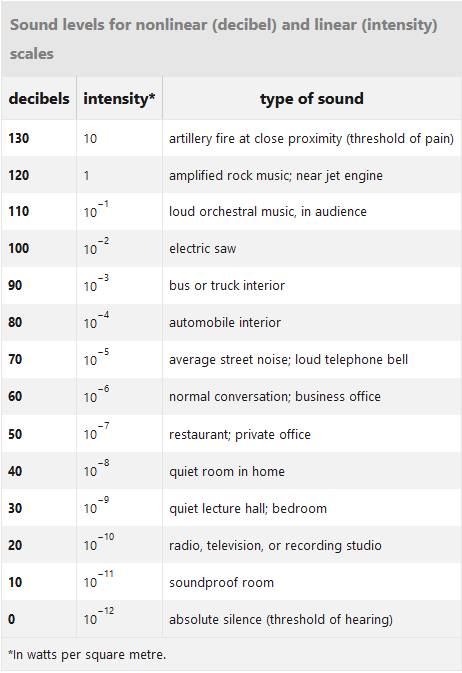
\includegraphics[scale=0.6]{img2.png}
\end{figure}

 Le champ auditif de l’être humain (en vert) est limité par une courbe qui nous fournis la limite inferieur et une autre courbe qui nous donne la limite supérieure de la perception sonore. A caque fréquence, entre $20 Hz et 20 kHz$, le seuil de notre sensibilité est différent. L’intervalle le plus large de perception a lieu aux alentours les $2 kHz$ et commence à partir des $0 dB$. Dans cet intervalle dit “moyen” les dynamiques sensorielles sont les plus aptes possibles et peuvent avoir un équivalent de $130 dB$.
 
% Imagen
 \begin{figure}[H]
 \centering
    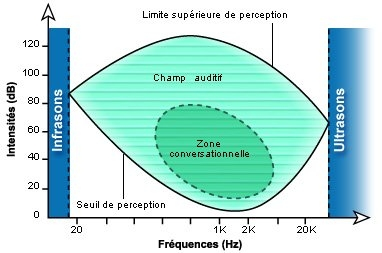
\includegraphics[scale=1.5]{img3.jpg}
    \caption{Courbe audiométrique de l'oreille humaine.}
\end{figure}

 \subsection{Tonalité pure}
 Lorsque nous utilisant de fonction comme celle de la vitesse de déplacement d’une onde, nous pouvons dire que cette fonction représente une tonalité pure avec un fréquence $f$. Ce nom dérive du fait que cette fonction décrit une onde sonore avec une seule composante en fréquence, c’est-à-dire qu’il s’agit d’un cas idéal, parce que en faisant analogie avec la lumière, dans la nature nous ne trouverons jamais une lumière monochromatique (d’une seule couleur, c’est-à-dire d’une seule fréquence), nous ne trouverons jamais une onde sonore avec cette caractéristique.  

Afin de donner une définition plus précise d’une tonalité pure, nous devons nous appuyer sur la définition donnée en psychoacoustique. En effet, en psychoacoustique, une tonalité pure, ou encore son pur ou note pure (en anglais : pure tone) est un son avec une forme d'onde sinusoïdale ; c'est-à-dire une onde sinusoïdale de n'importe quelle fréquence, phase et amplitude. En audiologie clinique, les tons purs sont utilisés pour l'audiométrie tonale (en) afin de caractériser les seuils d'audition à différentes fréquences. 

\subsection{Descomposición del sonido en tonos puros}
Proprement dit, toute onde sonore resulte de l’addtion de plusieurs tonalité pure de frequence differente. La quantite de 

Formalmente, cualquier sonido $f$ es una suma de tonos puros a diferentes frecuencias. La cantidad de cada frecuencia requerida para formar el sonido $f$ es el contenido frecuencial de $f$. Cualquier sonido puede ser reconstruido partiendo de su contenido frecuencial.

Una implicación de lo anterior es que, en general, cualquier sonido puede ser considerado como una función, y por más complejo que sea el sonido, puede ser representado por la suma de tonos puros o funciones sinusoidales (senos y cosenos) lo cual no es sorpresa que esté relacionado con el concepto matemático de series de Fourier. 

Adicionalmente, lo anterior también implica que el sonido $f$ puede ser almacenado al guardar simplemente su contenido frecuencial, como una alternativa de guardar a $f$ como tal.

\subsection{Espectro del sonido}
Le spectre en fréquences montre les différentes fréquences présentes dans un son, c’est-à-dire, il montre le contenue fréquentiel qui caractérise le son et avec l’amplitude correspondante à chaque fréquence. Usuellement, il est présenté comme un graphique où on compare la fréquence avec l’intensité, la pression ou la puissance en $dB$. Il faut remarquer que la fréquence dominante (avec une amplitude plus grande que les autres) est connue comme fréquence fondamentale et le reste est connue comme harmoniques. Sur l’image ci-dessous, on peut observer le spectre en fréquence d’une flute qui joue la note G4 équivalente, approximativement, a une fréquence de $400 Hz$. Il est important de remarquer que la fréquence fondamentale c’est celle qui a la plus grande amplitude, les autres ce sont des harmoniques. Si on étudiait cette note dans un autres instrument musical, on obtiendra le même spectre en fréquence avec la même fréquence fondamentale , mais les harmoniques seraient différents. Cette dernière caractéristique explique pourquoi les êtres humains on perçoit chaque instrument d’une façon différente lorsqu’on joue une même note. Cette perception auditive est connue sous le nom de \underline{timbre}.

% Imagen
 \begin{figure}[H]
 \centering
    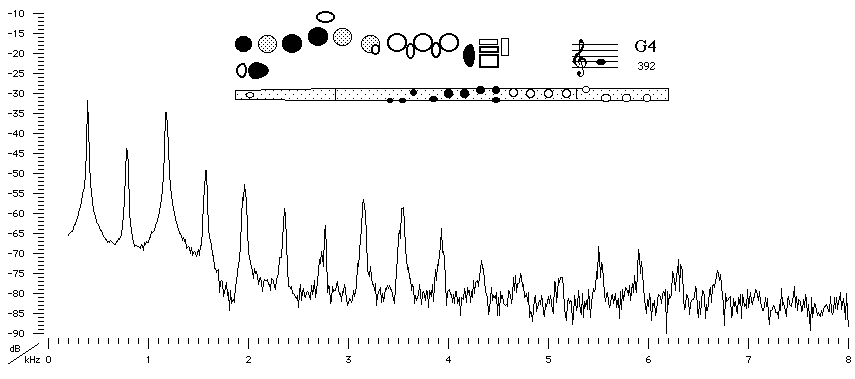
\includegraphics[scale=0.5]{img4.png}
    \caption{Spectre en fréquence du son d'une flute jouant la note G4 qui correspond, approximativement, à une fréquence de 400 Hz. On observe la fréquence fondamentale avec la plus grande amplitude et la présence des harmoniques}
\end{figure}

\subsection{Son digital}

L'échantillonnage d'un signal continu est l'opération qui consiste à prélever des échantillons du signal pour obtenir un signal discret, c'est-à-dire une suite de nombres représentant le signal, dans le but de mémoriser, transmettre, ou traiter le signal. 

L'échantillonnage intervient dans l'opération de conversion analogique-numérique, par exemple dans un dispositif de numérisation du son ou de l'image. Un autre exemple d'échantillonnage est celui que l'on fait pour obtenir la représentation graphique d'une fonction à une ou deux variables. D'une manière générale, l'échantillonnage intervient dans toute opération de conversion continu/discret. 

Le théorème de l'échantillonnage de Shannon, qui permet de savoir à quelle fréquence minimale il faut échantillonner un signal pour ne pas perdre l'information qu'il contient. 

Soit $u(t)$ une fonction représentant un signal continu. On considère un échantillonnage périodique défini par : 

où $k$ est un entier. Te est la période d'échantillonnage. $f_e=1/T_e$ est la fréquence d'échantillonnage. 

Le théorème de Shannon ([1]) concerne les signaux dont le spectre possède une fréquence maximale $f_{max}$, que l'on appelle des signaux à bande limitée. Par exemple, si $u(t)$ est un polynôme trigonométrique, la fréquence maximale est celle de la plus grande harmonique.

\textbf{Théorème de Shannon} : pour que le signal puisse être entièrement reconstruit à partir des échantillons, il faut et il suffit que : 

La fréquence d'échantillonnage doit être strictement supérieure à deux fois la plus grande fréquence présente dans le spectre du signal continu (condition de Nyquist-Shannon). Si cette condition est vérifiée alors : 

où la fonction sinus cardinale est définie par : 

Cette relation montre que le signal peut être reconstruit à partir des échantillons, ce qui signifie que toute l'information présente dans le signal original est conservée dans les échantillons. Nous verrons plus loin comment l'opération de reconstruction est effectuée en pratique. 

La moitié de la fréquence d'échantillonnage est appelée la fréquence de Nyquist $f_n$ et la condition de Nyquist-Shannon s'écrit donc $f_{max}<f_n$. 

Lorsque la condition n'est pas vérifiée, on dit qu'il y a sous-échantillonnage. On parle de sur-échantillonnage lorsque la fréquence de Nyquist est beaucoup plus grande que $f_max$. 

Le temps écoulé entre 2 échantillons successifs est connu comme période d’échantillonnage et est noté $T_s$. La longueur du vecteur est connue, usuellement, comme $N$ et a pour indices les numéros compris entre $0$ et $N-1$. Le processus de convertir une onde sonore(audio analogique) en un son digital est connue comme quantification de l’audio où à chaque échantillon on associe une valeur en amplitude (usuellement compris entre $-1$ et $1$). Le rand des possibles niveaux de l’amplitude, en d’autres mots,  le numéro d’échantillons équidistant de l’intervalle de valeurs d’amplitude $[-1, 1]$ est connue comme profondeur de couleur, par exemple :

\[8-bit = 2^8 = 256 \quad possibles valeurs\]
\[16-bit = 2^{16} = 65536 \quad possibles valeurs\]

Dans la figure ci-dessous, on peut observer l’effet de la quantification de l’audio et l’influence de la fréquence d’échantillonnage et la profondeur de couleur.

% Imagen
 \begin{figure}[H]
 \centering
    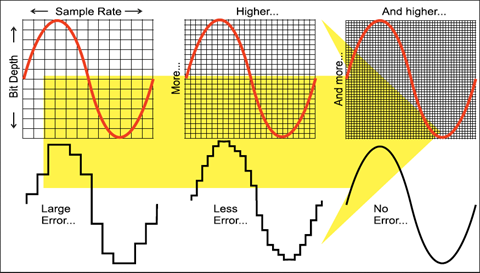
\includegraphics[scale=1]{img5.png}
    \caption{Cuantización de un sonido (audio análogo) y la influencia de la frecuencia de muestreo (Sample Rate) y la profundidad de bit (Bit Depth). Observe que entre mayor sean estos parámetros, mayor será el error cometido en la cuantización.}
\end{figure}

Comme on peut voir dans la figure ci-dessus, la fréquence d'échantillonnage et la profondeur de couleur jouent un rôle fondamental dans la détermination de la qualité de l'audio résultant.

\subsection{Monophonique}
 Un son monophonique, enregistré ou écouté en mono (apocope de monophonie), dit aussi monaural, n'est diffusé que sur un seul canal comme provenant d'une seule source ou d'un seul endroit. Il est en général enregistré par un seul microphone et reproduit par un ou plusieurs haut-parleurs diffusant le même signal acoustique.
 
\subsection{Son stéréo}
Le son stéréophonique, plus communément appelé stéréo, est une méthode de reproduction sonore visant à reconstituer la répartition dans l'espace des sources d'origine1.

Ce relief sonore est habituellement obtenu à l'aide de deux canaux (gauche et droit) diffusés par au moins deux transducteurs (haut-parleurs ou écouteurs). Dans des conditions idéales, l'auditeur entend les sons comme dans la nature ou comme s'il était situé en face de l'orchestre lors d'un concert.

Le terme stéréophonie vient du grec Stéréo « spatial, solide » et phono « ton, le son ».

\subsection{Enregistrement d'un son digital sur un ordinateur}
Usuellement sur un ordinateur, on utilise la méthode de modulation par impulsions codifié (PCM, Pulse-code modulation en anglais) pour transformer un signal analogue en une séquence de bits (signal digital). Cette méthode a été inventé par Alec Reeves en 1937 et est la forme standard des enregistrement audios digital sur les ordinateurs
Pour qu’un ordinateur soit capable de reproduit un son digital, il faut que les échantillons obtenus soient sauvegardés dans un fichier ou dans la mémoire de l’ordinateur. Dans le cas du PCM, l’enregistrement se fait sous format RAW ou en autres types de format (WAV, AIFF, AU…). Néanmoins, comme les fichiers audios sont grand, ce qui est normal est de travailler avec des formats compressés qui réduisent la taille des fichiers.

\begin{itemize} % Lista

    \item[-] \textbf{formats avec des pertes} \textit{(lossy)}:  il s’agit de formats qui compressent le fichier original en éliminant des parties de celui-ci en suivant un algorithme de compression spécifique. De ce fait, lorsqu’on décompresse le fichier, on n’obtient pas le fichier original. Certains d’entre eux sont: \texttt{MP3, Opus, Vorbis, WMA,} etc.
    \item[-] \textbf{Formats sans pertes} \textit{(lossless)}: il s’agit der format qui compresse le fichier original en organisant l’information efficacement. De ce fait, lorsqu’on décompresse le fichier on obtient l’original. Certains d’entre eux sont : \texttt{FLAC, APE, WV, ALAC,} etc.

\end{itemize}

\subsection{Audio en Matlab}
En Matlab la lectura de audios se realiza con la función:
\[\texttt{[y,Fs] = audioread('name.wav')}\]
Donde
\begin{itemize}
    \item[] $\texttt{y}$ es una matriz de $m$ filas y $n$ columnas donde $m=f*$\textit{durée} y $n$ depende del número de canales del audio (1 para mono, 2 para estereo). Los valores almacenados están en el intervalo $[-1,1]$ correspondiendo a la representación de un audio en el computador.
    \item[] $\texttt{Fs}$ es la frecuencia de muestreo del audio
\end{itemize}
En Matlab la escritura de audios se realiza con la función:
\[\texttt{audiwrite('name.wav',y,Fs)}\]

\subsection{Bruit et types de bruit}
Comme vue précédemment, le bruit dans un signal sonore correspond à une perturbation de celui-ci entrainant des pertes de d’information. Il existe plusieurs types de bruit qui ont leurs propres domaines de fréquences et qui altèrent ou modifient l’information contenue dans un signal de façon différente. En effet, entre les différents types de bruits nous pouvons remarqués 2 groupes très importants : Les bruits dit naturels et les bruits dit industriels.  

Dans un premier temps, en regardant les bruits naturels nous pouvons nous rendre compte que ces bruits ne sont pas produits de façon artificielle et existe par différentes raisons. Dans cette famille de bruit nous pouvons trouvés le bruit ambiant qui correspond au bruit total existant dans une situation donnée pendant un intervalle de temps donné, ainsi que les bruits qui le compose telles que le bruit résiduel et le bruit particulier. De plus, nous trouvons aussi des bruits dis colorées telles que le bruit blanc ou le bruit rose, qui feront objet de notre étude de filtrage. Tout d’abord, il faut remarquer que le bruit blanc est un bruit composé par la somme de tous le bruit coloré, c’est à dire l’addition en fréquence du bruit rose, bruit rouge ou brownien, bruit bleu ou azur, bruit violet et bruit gris. Chacun d’entre eux aillant un domaine de fréquence particulier et des caractéristique propre. Par exemple :\\

 % Imagen
    \begin{figure}[H]
        \centering
        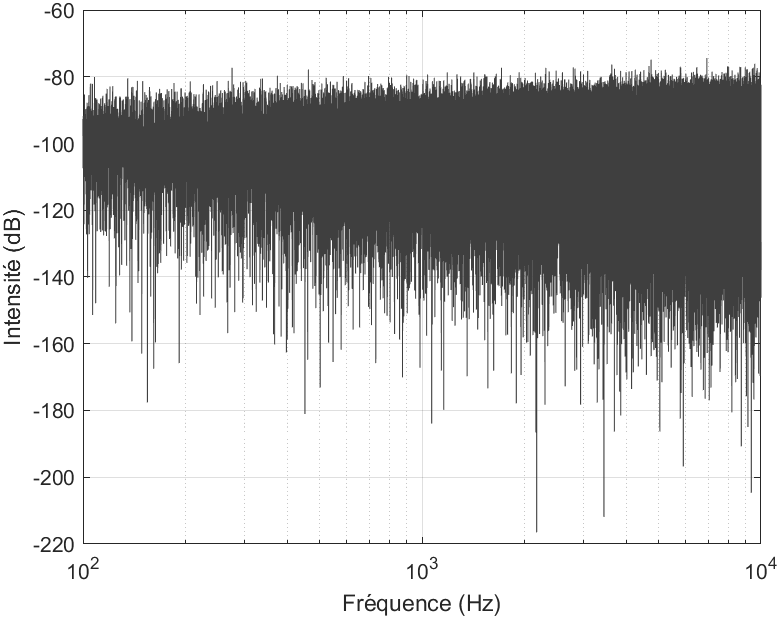
\includegraphics[scale=0.5]{img6.png}
        \caption{Spectre en frequence du bruit blanc généré sur Matlab R2020a.}
    \end{figure}
    
\begin{itemize} % Lista

    \item[-] \textbf{Le bruit rouge ou brownien} correspond dans une première approximation, dans les domaines qui utilisent des définitions précises, la terminologie « bruit rouge », « bruit brownien » ou « bruit brun » fait référence au son ayant une puissance sonore qui décroît de 6 dB par octave lorsque la fréquence augmente (densité proportionnelle à 1/f ) sur un intervalle de fréquence n'incluant pas de DC (Qui dans un sens général, n'inclut pas de composante constante, ou de valeur pour f=0). 

    % Imagen
    \begin{figure}[H]
        \centering
        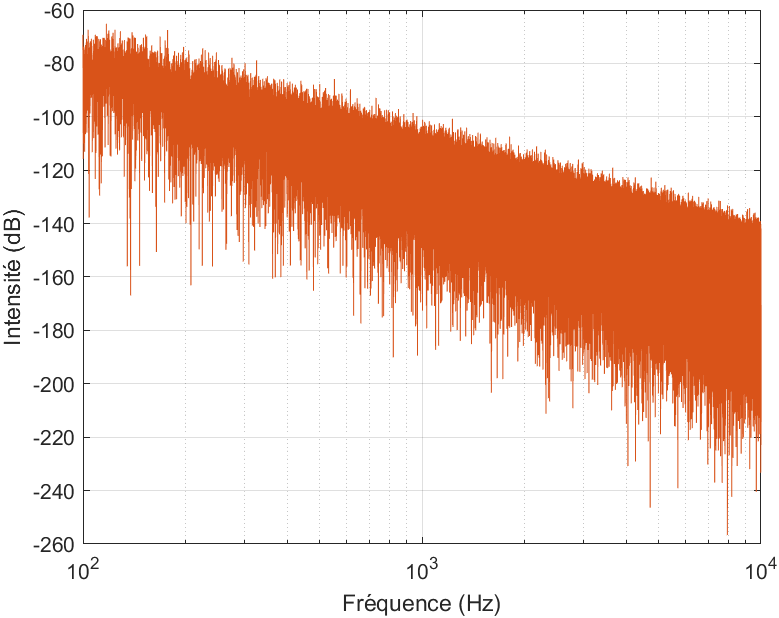
\includegraphics[scale=0.5]{img7.png}
        \caption{Spectre en fréquence du bruit rouge (-$6dB$/Octave) généré sur Matlab R2020a.}
    \end{figure}

    D’un autre point de vue, dans les domaines qui utilisent des définitions plus approximatives, le « bruit rouge » correspond à tout son dont la densité de puissance diminue lorsque la fréquence augmente3. 

    Plus exactement Le bruit rouge, peut être obtenu en utilisant un algorithme simulant le mouvement brownien ou par intégration mathématique du bruit blanc.
    
    \item[-] \textbf{Le bruit rose} Le spectre sonore du bruit rose est plat dans un espace logarithmique. Ainsi, ce type de bruit est caractérisé par une puissance égale sur des bandes proportionnelles en largeur. Une bande correspond en fait à un changement de fréquence (hausse ou baisse à exprimer en pourcentage de l’une des extrémités de l’intervalle). Par exemple, la puissance d’un bruit rose est la même sur les intervalles allant de $40$ à $60 Hz$ et de $4 000$ à $6 000 Hz$ car ces intervalles sont proportionnels (ils correspondent à une hausse de 50\% de la fréquence).

    Or, l’appareil auditif humain est souvent étudié dans un espace logarithmique. En effet, l’oreille humaine ne perçoit les sons que sur des bandes de largeurs proportionnelles : un doublement de fréquence sera perçu en termes de puissance sonore de la même façon, quelle que soit la fréquence de départ. Ainsi, en musique, on a défini les octaves : une octave correspond à un doublement de fréquence et est perçu comme contenant la même puissance sonore. C’est pourquoi le bruit rose est souvent utilisé comme signal de référence en ingénierie du son.
    
    D’autre part, sur les diagrammes de spectres sonores, on voit que la densité de puissance sonore du bruit rose, comparée à celle du bruit blanc, diminue de 3 dB par octave : la densité de puissance sonore est proportionnelle à $1/F$ (où $F$ est la fréquence). C’est pour cela que le bruit rose est souvent appelé « bruit $1/F$ ».
    
    % Imagen
    \begin{figure}[H]
        \centering
        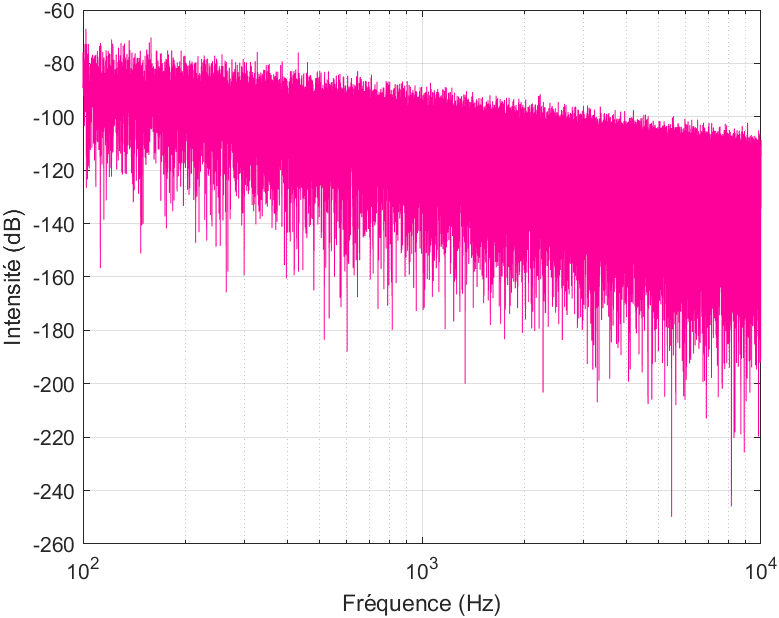
\includegraphics[scale=0.5]{img8.png}
        \caption{Spectre en fréquence du bruit rose (-$3dB$/Octave) généré su Matlab R2020a.}
    \end{figure}

    \item[-] \textbf{Le bruit bleu} qui correspond à un bruit qui augmente sa puissance sonore de 3 dB par octave lorsque la fréquence augmente (densité proportionnelle à f), et ce jusqu’à une fréquence infinie. 

    Dans le domaine de l’informatique graphique, le terme « bruit bleu » est parfois utilisé d’une façon plus approximative pour décrire tout son de puissance sonore minimale à basse fréquence et ne présentant aucun pic lorsque la fréquence augmente (croissance constante). 

    Il est convenable de connaitre et différencier aussi le bruit rose des autres types de bruits coloré, dans la mesure que ce type de bruit fait partie de notre étude. Donc le bruit rose, ce type de bruit est caractérisé par une puissance égale sur des bandes proportionnelles en largeur. Une bande correspond en fait à un changement de fréquence (hausse ou baisse à exprimer en pourcentage de l’une des extrémités de l’intervalle). Par exemple, la puissance d’un bruit rose est la même sur les intervalles allant de 40 à 60 Hz et de 4000 à 6000 Hz car ces intervalles sont proportionnels (ils correspondent à une hausse de 50 pourcent de la fréquence). 

\end{itemize}
\hfill

Dans un deuxième temps, nous voyons l’existence d’une deuxième
famille de bruits que nous choisissant de nommé des bruits
industriels. En effet, comme son nom l’indique les bruits
industriels sont des perturbations sonores produits par l’industrie
ou par des effet industrie. Dans cette famille nous trouvons des
bruits tels que le bruit de route qui est un bruit normalisé. Il est
une référence pour le bruit des trafics routiers et ferroviaires.
Son spectre est enrichi en basses fréquences et appauvri dans les
aiguës par rapport à un bruit rose. Mais aussi nous trouvons des
bruits comme les suivants :
\hfill

\begin{itemize}

    \item[-] \textbf{Le bruit d’impact}: c’est le bruit transmis par une paroi mise en vibration par un choc (bruit de pas, déplacement de meubles, chute d’objet, enfoncement d’un clou dans un mur...).
    \item[-] \textbf{Le bruit aérien}: c’est le bruit propagé dans l’air (bruit de voix, bruit de télévision, bruit de circulation...). 
    \item[-] \textbf{Le bruit solidien}: c’est le bruit propagé dans les milieux solides comprenant (le bruit d’impact transmis par les éléments solides, le bruit d’équipement (chaufferie, ascenseurs, ...). 
    
\end{itemize}

\newpage
\section{Méthodes}
Le but de ce projet est de implementer le filtrage dans les notes audios dans l'objectif d'attenuer le bruit present. Pour cela nous allons implementé le filtrage analogique avec une approximation de Butterworth, la méthode RNN et un autre qui reste définir.

\subsection{\textbf{Filtre de Butterworth}}

\subsubsection{definition du filtrage}
\medskip
Le filtrage est une forme de traitement de signal, obtenu en envoyant le signal à travers un ensemble de circuits électroniques, qui modifient son spectre de fréquence et/ou sa phase et donc sa forme temporelle. Il peut s‘agir soit : 

\begin{itemize}
    \item[-] d’éliminer ou d’affaiblir des fréquences parasites indésirables 

    \item[-] d’isoler dans un signal complexe la ou les bandes de fréquences utiles. 
\end{itemize}

Il existe plusieurs types de filtres : passe-bas, passe-haut, passe-bande, coupe-bande, passe-tout. Dans notre étude, nous allons nous concentrer dans les filtres passe-bas.

\medskip
\subsubsection{Filtre passe-bas}
Un filtre passe-bas est un filtre qui laisse passer les basses fréquences et qui atténue les hautes fréquences, c'est-à-dire les fréquences supérieures à la fréquence de coupure. Il pourrait également être appelé filtre coupe-haut. Le filtre passe-bas est l'inverse du filtre passe-haut et ces deux filtres combinés forment un filtre passe-bande. 

Un filtre passe-bas peut être implémenté de façon analogique avec des composants électroniques. Ainsi, ce genre de filtre s'applique sur des signaux continus en temps réel. Les composants et la configuration du circuit fixeront les différentes caractéristiques du filtre, telles que l'ordre, la fréquence de coupure et son diagramme de Bode. Les filtres analogiques classiques sont du premier ou du second ordre. Il existe plusieurs familles de filtres analogiques : Butterworth, Tchebychev, Bessel, elliptique, etc. L'implémentation des filtres de même famille se fait généralement en utilisant la même configuration de circuit, et ceux-ci possèdent la même forme de fonction de transfert, mais ce sont les paramètres de celle-ci qui changent, donc la valeur des composants du circuit électrique.
\medskip

\paragraph{Filtre passe-bas du premier ordre}
Un filtre passe-bas du premier ordre est caractérisé par sa fréquence de coupure $f(c)$.  La fonction de transfert du filtre est obtenue en dénormalisant le filtre passe-bas normalisé en en remplaçant $\omega_n$ par $\omega$ $\omega_c$,
ce qui donne la fonction de transfert suivante :

\begin{equation}
    H(j\omega)= \frac{v_o}{v_i} = \frac{K}{1+j\frac{\omega}{\omega_c}}
\end{equation}

où
\begin{itemize}
    \item[] $v_i$ est le signal d'entrée
    \item[] $v_0$ est le signal de sortir
\end{itemize}


Le module et la phase de la fonction de transfert sont égaux à :

\begin{equation}
    |H(\omega)|=|\frac{v_o}{v_i}|= \frac{K}{\sqrt{1 + (\frac{\omega}{\omega_c})^2}}
\end{equation}

\begin{equation}
    \phi(\omega) = arg(H(j\omega)) = -arg(1 + j\frac{\omega}{\omega_c}) = \arctan(\frac{\omega}{\omega_c})
\end{equation}

Il y a plusieurs méthodes pour implémenter ce filtre. Une réalisation active et une réalisation passive sont ici présentées. K est le gain du filtre.

\paragraph{Circuit actif}
\hfill\\
Il est  possible de réaliser un filtre passe-bas avec un circuit actif. Cette option permet d'ajouter du gain au signal de sortie, c'est-à-dire d'obtenir une amplitude supérieure à 0 dB dans la bande passante. Plusieurs configurations permettent d'implémenter ce genre de filtre.

%imagen
 \begin{figure}[H]
 \centering
    \includegraphics[scale=0.5]{Circuit.png}
    \caption{Un filtre passe-bas actif}
\end{figure}

Un filtre passe-bas actif
Dans la configuration présentée ici, la fréquence de coupure se définit comme suit :

\begin{equation}
    f_c = \frac{1}{2\pi R_2C} ou  \omega_c = \frac{1}{R_2 C}
\end{equation}

En utilisant les propriétés des amplificateurs opérationnels, et les impédances des éléments, on obtient la fonction de transfert suivante :

\begin{equation}
    H(j\omega)= \frac{v_o}{v_i} = \frac{-R_2}{R_1} \cdot \frac{1}{1 + jR_2 C\omega}
\end{equation}

En basse fréquence, le condensateur agit comme un circuit ouvert, ce qui est confirmé par le fait que le terme de droite de l'équation précédente tend vers 1. La formule simplifiée ainsi obtenue nous donne le gain dans la bande passante :

\begin{equation}
    H(\omega)_{\omega \ll \omega_c}  = \frac{v_o}{v_i} = \frac{-R_2}{R_1}
\end{equation}


Avec la fonction de transfert, on peut démontrer que l'atténuation dans la bande rejetée est de 20 dB/décade ou de 6 dB par octave telle qu'attendu pour un filtre d'ordre 1.
\medskip

\paragraph{Filtre passe-bas du second ordre}
\hfill\\
Un filtre passe-bas du secon ordre est caractérisé par sa fréquence propre $f_0$ et par un facteur de qualité Q.  Il est représenté par la fonction de transfert suivante :


\begin{equation}
    H(j\omega) = \frac{v_o}{v_i} = \frac{K}{1 - (\frac{\omega}{\omega_0})^2 + j\frac{(\frac{\omega}{\omega_0})}{Q}}
\end{equation}

avec
\begin{itemize}
  \item[] $\omega =  2\pi f$
  \item[] $\omega_0 = 2\pi f_0$ 
\end{itemize}


Le module et la phase de la fonction de transfert sont donc donnés par:

\begin{equation}
    |H(j\omega)| = |\frac{v_o}{v_i}| = \frac{K}{\sqrt{(1 - (\frac{\omega}{\omega_0})^2)^2 + (\frac{(\frac{\omega}{\omega_0})}{Q})^2}}
\end{equation}

\begin{equation}
    \phi(\omega) = -arctan(\frac{\frac{(\frac{\omega}{\omega_0})}{Q}}{1 - (\frac{\omega}{\omega_0})^2})
\end{equation}

\subsubsection{Types de Filtres Analogiques Passe-bas}
\paragraph{Approximation de Butterworth}
\hfill \\
Un filtre de Butterworth est un type de filtre linéaire, conçu pour posséder un gain aussi constant que possible dans sa bande passante.

Les filtres de Butterworth furent décrits pour la première fois par l'ingénieur britannique Stephen Butterworth

\begin{itemize}
  \item[-] \textbf{Caractéristiques}
  Le gain d'un filtre de Butterworth est le plus constant possible dans la bande passante et tend vers 0 dans la bande de coupure. Sur un diagramme de Bode logarithmique, cette réponse décroît linéairement vers -$\infty$, de -6 dB/octave (-20 dB/décade) pour un filtre de premier ordre, -12 dB/octave soit -40 dB/decade pour un filtre de second ordre, -18 dB/octave soit -60 dB/decade pour un filtre de troisième ordre, etc.
  
  %Imagen
  \begin{figure}[H]
 \centering
    \includegraphics[scale=0.5]{Filter.jpeg}
    \caption{Gains de filtres de Butterworth passe-bas d'ordre 1 à 5 en fonction de la fréquence}
\end{figure}
  
  \item[-] \textbf{Fonction de Transfert}
  Le gain d'un filtre de Butterworth passe-bas d'ordre n est :
  
  \begin{equation}
      G_n(\omega) = |H(j\omega)| = \frac{1}{\sqrt{1 + (\frac{\omega}{\omega_0})^2}}
  \end{equation}

\end{itemize}

Avec
\begin{itemize}
    \item[] $G_n$ est le gain du filtre.
    \item[] $H_n$ sa fonction de transfert.
    \item[] $j$ l'unité imaginaire $j^2 = -1$
    \item[] $\omega$ la fréquence angulaire (ou pulsation) du signal en radians par seconde ($\omega = 2\pi f$
    \item[] et $\omega_c$ la fréquence de coupure (angulaire) du filtre (à -3dB).
\end{itemize}
En normalisant l'expression (c’est-à-dire en spécifiant $\omega_c = 1$):

\begin{equation}
    G_n(\omega) = |H(j\omega)| = \frac{1}{\sqrt{1 + \omega}^2}
\end{equation}

Les 2n-1 premières dérivées de $G_n$ sont nulles pour $\omega = 0$, impliquant une constance maximale du gain dans la bande passante.

Aux hautes fréquences :

\begin{equation}
    |H(j\omega)|_{dB} \approx -20 \cdot n\log_{10}(\omega)
\end{equation}
Le roll-off du filtre (la pente du gain dans un diagramme de Bode) est de -20n dB/décade, où 'n' est l'ordre du filtre.

Le gain ne représente que le module de la fonction de transfert $H(p)$ (au sens de la transformée de Laplace), ce qui laisse une certaine latitude pour déterminer cette dernière. On doit avoir

\begin{equation}
    H(p)H(-p) = \frac{G_0^2}{1 + (-\frac{p^2}{\omega_c^2})^n}
\end{equation}

Les pôles de cette expression sont équirépartis sur un cercle de rayon  $\omega_c$. Pour que le filtre soit stable, on choisit les pôles de la fonction de transfert comme ceux de $H(p)H(-p)$ ayant une partie réelle négative. Le k-ième pôle est donné à l'aide des racines n-ièmes de l'unité :

\begin{equation}
    -\frac{p_k^2}{\omega_k^2} = \exp({\frac{j(2k - 1)\pi}{n}}); k = 1,2,3,...,n
\end{equation}
    

d'où

\begin{equation}
    p_k = \omega_c\exp{\frac{j(2k + n - 1)\pi}{2n}};  k = 1,2,3,...,n
\end{equation}

La fonction de transfert s'écrit en fonction de ces pôles :

\begin{equation}
    H(p) = \frac{G_0}{\prod{n=1}^{n}\frac{(p - p_k)}{\omega_c}}
\end{equation}

Le polynôme au dénominateur est appelé polynôme de Butterworth.

\begin{center}
    \begin{tabular}{|| c c||}
    \hline
    n & Polynôme de Butterworth $B_n(p)$ pour $w_c = 1$ \\ [0.5ex]
    \hline \hline
    1 & $(p + 1)$ \\
    \hline
    2 & $p^2 1.4142p + 1$ \\
    \hline
    3 & $(p + 1)(p^2 + p + 1)$ \\
    \hline
    4 & $(p^2 + 0.7654p + 1)(p^2 + 1.8478p + 1)$ \\
    \hline
    5 & $(p + 1)(p^2 + 0.6180p + 1)(p^2 1.6180p + 1)$ \\
    \hline
    6 & $(p^2 + 0.5176p + 1)(p^2 + 1.4142p + 1)(p^2 + 1.9319p + 1)$ \\
    \hline
    7 & $(p + 1)(p^2 0.4450p 1)(p^2 + 1.2470p + 1)(p^2 + 1.8019p + 1)$ \\
    \hline
    8 & $(p^2 + 0.3902p + 1)(p^2 + 1.1111p + 1)(p^2 + 1.6629p + 1)(p^2 + 1.9616 + 1)$ \\ [0.1ex]
    \hline
    \end{tabular}
\end{center}




Les polynômes normalisés de Butterworth peuvent être utilisés pour déterminer les fonctions de transfert de filtre passe-bas pour toute fréquence de coupure $\omega_c$ selon que:

\begin{equation}
    H(p) = \frac{G_0}{B_n(a)}, a = \frac{p}{\omega_c}
\end{equation}

\paragraph{Approximation de Tchebychev}
\hfill
\medskip
\begin{itemize}
    \item[-] \textbf{Fonctionde Transfert:}
    Les filtres Chebyshev de type I sont les types les plus courants de filtres Chebyshev. La réponse en gain (ou en amplitude ) , en fonction de la fréquence angulaire du filtre passe-bas du n ième ordre est égale à la valeur absolue de la fonction de transfert évaluée à $G_n(s)\omega H(s)s = j\omega$

        \begin{equation}
            G_n(s) = |H_n(j\omega)| = \frac{1}{\sqrt{1 + \epsilon^2T_n^2(\frac{\omega}{\omega_0})}}
        \end{equation}

        où $\epsilon$ est le facteur d'ondulation,$\omega_0$ est la fréquence de coupure et $T_n$ est un polynôme de Chebyshev du $n$-ème ordre
    
        \item[-] \textbf{Polynme de Tchebychev:}
        La définition classique des polynômes de Tchebychev de première espèce est le plus souvent donnée par la relation de récurrence suivante :

            \begin{equation}
                T_{n+1} = 2XT_n - T_{n1}; \forall n \geq 0; T_0 = 1;  T_1 = X
            \end{equation}
 
\end{itemize}


\paragraph{Filtre de Bessel}
\hfill
\medskip
\begin{itemize}
    \item[-] \textbf{Fonctionde Transfert:}
    Un filtre passe-bas Bessel se caractérise par sa fonction de transfert :

        \begin{equation}
            H(s) = \frac{\Theta_n(0)}{\Theta_n(s/\omega_0)}
        \end{equation}

    où $\Theta_n(s)$ est un polynôme de Bessel inversé dont le filtre tire son nom et $\omega_0$ est  la fréquence de coupure . Le filtre a un retard de groupe basse fréquence de $1/\omega_0$. Puisque est indéterminé par la définition des polynômes de Bessel inversés, mais $\Theta_n(0)$ est une singularité amovible, il est défini que $\Theta_n(0) =  \lim_{x\to\infty} \Theta_n(x)$

    \item[-] \textbf{Polynôme de Bessel:}
        Les polynômes de Bessel inversés sont donnés par: 

        \begin{equation}
            \Theta_n(s) =  \sum_{k=0}^{n} a_k s^k 
        \end{equation}

        où

        \begin{equation}
            a_k = \frac{(2n - k!)}{2^{n-k} k!(n-k!)}; k = 1,2,3,...,n
        \end{equation}
\end{itemize}

\subsubsection{Notions Importantes}
\paragraph{Diagramme de Bode}
Le diagramme de Bode d'un système de réponse fréquentielle $T(j\omega)$ se compose de deux tracés:

\begin{itemize}
    \item[-] le gain (ou amplitude) en décibels (dB). Sa valeur est calculée à partir de $20\log_{10}(|T(j\omega|)$

    \item[-] la phase en degré, donnée par $arg(T(j\omega))$
\end{itemize}

L'échelle des pulsations est logarithmique et est exprimée en rad/s (radian par seconde). L'échelle logarithmique permet un tracé très lisible, car construit à partir de tronçons de ligne droite.

%imagen
%diagramme de Bode
\begin{figure}[H]
 \centering
    \includegraphics[scale=0.3]{Bode.jpeg}
\end{figure}

\paragraph{Transformée de Laplace}
La transformée de Laplace d’une fonction f(t) est :
\begin{equation}
    F(s) = L{f(t)} = \int\limits_{0}^{\infty}\ f(t)\exp(-st) dt
\end{equation}

La transformée de Laplace permet de transformer le problème du domaine du temps au domaine de fréquence.
Lorsqu’on obtient la réponse voulue dans le domaine de fréquence, on transforme le problème á nouveau dans le domaine du temps, á l’aide de la transformée inverse de Laplace, qui est definie par:

\begin{equation}
    f(t) = L^{-1}{F(s)} = \frac{1}{2j\pi} \int\limits_{-\infty}^{\infty} \ F(s)\exp(st) ds
\end{equation}

\subsection{\textbf{Filtre de Wiener}}
Le filtre de Wiener est une des meilleur filtres linaires de minimum carré. Il peut être utilisé pour prédire, estimer, interpoler, filtrer un signal et le bruit, entres autres. Pour créer ce type de filtre, il faut connaitre avoir une connaissance préalable du signal que le système aura comme entrée, c’est à dire le signal qui sera filtré. Le plus grand problème c’est que cette information est difficile à obtenir, c’est pour cela que les filtres adaptatifs sont très importants, parce qu’ils utilisent les données d’entrée pour pouvoir déterminer les données statistiques requis. En général, on a un signal $f(k)$, une réponse désiré $d(k)$ et un filtre linéaire de réponse impulsionnelle $h(k)$. Ce filtre est alimenté par $f(k)$ et produit une sortie $g(k)$. La différence entre le signal de sortie $g(k)$ et le signal désiré $d(k)$, est connue comme erreur d’estimation $e(k)$, la figure suivante illustre ce fait :

% Imagen

\begin{figure}[H]
 \centering
    \includegraphics[width=0.5\textwidth]{Wiener.png}
    \caption{Filtre de Wiener}
\end{figure}

L’objectif du filtre de Weiner est de déterminer la réponse impulsionnelle $h(k)$ dans le but de produit une erreur $e(k)$ le plus petit possible. Le critère utiliser pour réaliser cela est la minimalisation du valeur quadratique moyen de l’erreur.

Le filtre digital montrer dans l’image a un signal d’entre et produit un signal de sortie. Le filtre sera un filtre de Wiener si sa réponse impulsionnelle est choisie dans l’objectif de minimiser l’erreur quadratique moyen. L’erreur est définie comme la différence entre la sortie et la réponse désiré et est décrit par l’équation suivante :
\begin{center}
     $e_k=d_k-g_k$
\end{center}{}

Lorsque nous travaillons avec le filtre de Weiner, généralement la réponse désirée existe dans la forme théorique. Cependant, dans ce cas on travaille avec un réponse désiré connue. La réponse impulsionnelle du filtre de Weiner est obtenue 

Si nous appliquons le carré a l’équation de l’erreur, nous avons :

% ecuación
\begin{center}
    $e_k^2=d_k^2+g_k^2-2d_kg_k$
\end{center}{}
    

Et on sait que :

% ecuación
\begin{center}
     $g_k$ =$\displaystyle\sum_{l=0}^{\infty}f_{k-l} h_l $
\end{center}


Si on substitue dans l’équation de l’erreur, on a :

% ecuación
\begin{center}
    $e_k^2=d_k^2+$ $\displaystyle \sum_{l=-\infty}^{\infty}\displaystyle\sum_{m=-\infty}^{\infty}$$h_l h_\mu f_{k-l} f_{k-\mu}$ $- 2$  $\displaystyle\sum_{l= -\infty}^{\infty}f_{k-l} h_l d_k$
\end{center}

Si, on prend la valeur moyenne à chaque côté, on trouve une expression pour l’erreur quadratique moyenne 

% ecuación
\begin{center}
     $E[e_k^2]=E[d_k^2]+$ $\displaystyle \sum_{l=-\infty}^{\infty}\displaystyle\sum_{m=-\infty}^{\infty}$$h_l h_\mu E[f_{k-l} f_{k-\mu}]$ $- 2$  $\displaystyle\sum_{l= -\infty}^{\infty}h_l E[f_{k-l}  d_k]$
\end{center}
\begin{center}
        $= \phi_{dd} (0) + $ $\displaystyle \sum_{l=-\infty}^{\infty}\displaystyle\sum_{m=-\infty}^{\infty}$ $h_l h_\mu \phi_{ff} (l-\mu)$  $- 2$  $\displaystyle\sum_{l= -\infty}^{\infty} h_l \phi_{fd}(l)$
\end{center}

Avec $\phi_{dd}$ et $\phi_{ff}$ l’autocorrélation et $\phi_{fd}$ la corrélation croisée entre les signaux $f$ et $d$. Si on dérive en fonction de $h$ et on cherche la solution de l’équation lorsque celle-ci tend vers $0$, on a :

% ecuación
\begin{center}
     $\displaystyle\sum_{l= -\infty}^{\infty}$ $h_l^* \phi_{ff} (j-l)=\phi_{fd}(j)$
\end{center}

Cette équation est l’équation de Wiener-Holpf, qui peut être écrit de la façon suivante, grave au produit de convolution :

% ecuación
\begin{center}
     $h_l^* * \phi_{ff} (k) = \phi_{fd} (k)$
\end{center}
Et si on applique la transformé en $Z$ a chaque partie de l’équation, on a :

% ecuación
\begin{center}
     $H^*(z) \phi_{ff}(z)=\phi_{fd}(z)$  ó  $H^*(z)=\frac{\phi_{fd}(z)}{\phi_{ff}(z)}$
\end{center}

Avec la solution de Weiner, on pet trouver la fonction de transfert du filtre $H(z)$ a partie de la transformé en $Z$ de la fonction d’autocorrélation d’un signal d’entrée, de la corrélation croisée du signal d’entré et la réponse désirée. Si on remplace cette équation dans l’expression de l’erreur, on a la valeur minimal MSE :

% ecuación
\begin{center}
     $E(e_k^2)_{min}=\phi_{dd}(0)-$ $\displaystyle\sum_{l= -\infty}^{\infty}h_l^* \phi_{fd}(l)$
\end{center}


\subsection{\textbf{RNNbruit: Méthode hybride DSP/Deep Learning}}
La méthode RRNbruit est une méthode créé para Jean-Marc Valin de Mozilla Corporation. Il s’agit d’une méthode hybride pour atténuer le bruit, en thermes général elle fonction de la façon suivante : elle utilise le Deep Learning dans des cas où la réduction du bruit demande réglage ou une configuration minutieuse, alors que pour les cas qui ne le demande pas, la méthode emplois des procèdes d’élimination du bruit classiques. Pour mieux comprendre le fonctionnement de ce filtre, nous allons étudier plus attentivement les concepts qui ont un rôle important dans cette méthode, tels que réseau de neurones artificiels, Deep Learning et réseau de neurones récurrentes.
\hfill\\

\subsubsection{Réseau de neurones artificiels}
Pour pouvoir comprendre de quoi il s’agit un réseau de neurones, il est convenable de commencer par un élément de ce réseau : un neurone artificiel. Il existe plusieurs modèles de neurones artificiels, cependant, il suffit de de définir le plus bas niveau, le perceptron, et le modèle le plus utilise dans les industries modernes, le sigmoïde. 
\hfill\\

\paragraph{Perceptron}
Les perceptrons ont été développer entre les années 1950 et 1960 par le scientifique Frank Rosenblatt, inspirée du travail réalisé par Warren McCulloch et Walter Pitts en 1943. 

Un perceptron prend plusieurs entrée binaires (uniquement de $0$ et de $1$) $x_1, x_2, ...$ et produit une unique sortie binaire, par exemple : 

%imagen
 \begin{figure}[H]
 \centering
    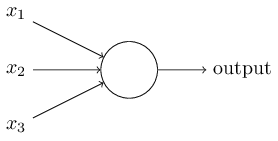
\includegraphics[scale=0.5]{img9.png}
    \caption{Ejemplo de la representación gráfica de un perceptrón.}
\end{figure}

Dans ce cas le perceptron a 3 entrées, amis en général il peut avoir une quantité arbitraire d’entrées, Rosenbatt propose une règle simple pour calculer la sortie. En effet, il introduit de poids $w_1, w_2, ...$ qui représentent des nombres réels illustrant l’importance de chaque entrée respectivement avec la sortie. La sortie de la neurone ($0$ ou $1$)  résulte de la somme pondérée des entrées, si cette somme est supérieure à une valeur limite, la sortie sera égale à $1$, mais si elle est inferieurs à cette valeur limite la sortie sera $0$. 

%ecuacion
\begin{equation}
    output =
    \begin{cases*}
      0 & if $\Sigma_j w_jx_j \leq $ threshold \\
      1 & if $\Sigma_j w_jx_j > $ threshold \\
    \end{cases*}
\end{equation}

La valeur limite est aussi un nombre réel. Il s’agit d’un paramètre du neurone. Pr notation, on simplifie la description précédant en considérant $w$ et $x$ comme des vecteurs des poids et des entrées, respectivement, donc la somme pondérée devient : 

%ecuacion
\begin{equation}
    w \cdot x \equiv \Sigma_j w_jx_j
\end{equation}

Finalement, on définit le biais noté b comme $b \equiv -$threshold, alors on a: 

%ecuacion
\begin{equation}
    output =
    \begin{cases*}
      0 & if $w \cdot x + b \leq 0$ \\
      1 & if $w \cdot x + b > 0$ \\
    \end{cases*}
\end{equation}

Il faut comprendre le biais comme un objet de mesure qui permet de déterminé à quel point il est facile de faire que la sortie du perceptron soit égale à $1$. En termes biologiques, le biais est une mesure qui permet de savoir à quel point il est facile de faire que le perceptron se déclenche ou s’active. 

Même si les perceptrons sont très utilisés pour modéliser une grande variété de problèmes, ils ont un grand désavantage. En effet, un petit changement dans le vecteur des biais ou dans celui des poids, peut entrer un grand changent dans la sortie, ce qui peut être problématique, même dans le cas d’un algorithme de bas niveau d’apprentissage.
\hfill\\

\paragraph{Neurones Sigmoïdes}
Elles se représentent de la même façon que les perceptrons : 

%imagen
 \begin{figure}[H]
 \centering
    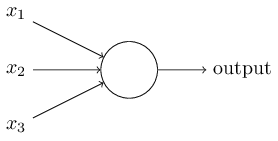
\includegraphics[scale=0.5]{img9.png}
    \caption{Ejemplo de la representación gráfica de un sigmoïde.}
\end{figure}

Elles ont un nombre arbitraire d’entrées $x_1, x_2, ...$, mais les valeurs des entrées prennent de valeurs comprises entre 0 et 1. Elles possèdent aussi un poids pour chaque entrée, $w1, w2, ...$, et un biais $b$. Dans ce cas, les sorties ne sont pas de valeurs de $0$ ou $1$, mais une fonction $g(w\cdot x+b)$, où g est appelé la fonction sigmoïde ou en général, fonction d’activation, et est définie par : 

%ecuacion
\begin{equation}
    g(z)=\dfrac{1}{1+e^-z}
\end{equation}

Où $z=w\cdot x+b$. Grafiquement est definie par:

%imagen
 \begin{figure}[H]
 \centering
    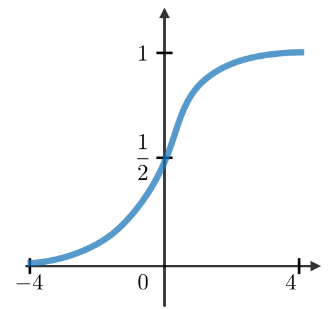
\includegraphics[scale=0.5]{img10.png}
\end{figure}

Dans ce cas, on observe que la sortie prend des valeurs entre $0$ et $1$, ceux qui revient à dire que la sortie peut prendre une infinité de valeurs. Usuellement, lorsqu’on emplois des sigmoïdes, l’intervalle est devisé en partitions et en fonction de la valeur obtenue, on fait une interprétation particulière de la sortie. Par exemple, en traitement d’image si on veut savoir si l’image d’entrée possède le numéro $9$, on pourrait employer une cote de $0.5$.  


\paragraph{Autres modèles de neurones utilisés dans le modèle}
La méthode RNNbruit emploie des réseaux de neurones avec de neurones sigmoïdes mais il peut employer deux autres modèles de neurones : $Tanh$ et $RELU$. Le comportement et la description de ces modèles est exactement le même, avec un changement de la fonction d’activation $g$. 

%imagen
 \begin{figure}[H]
 \centering
    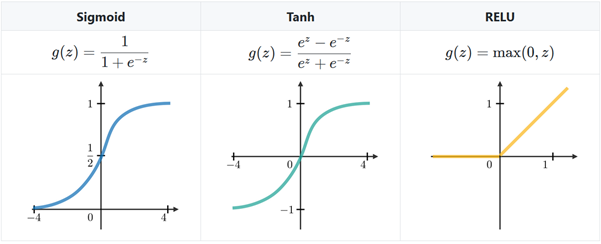
\includegraphics[scale=0.7]{img11.png}
\end{figure}


\subsubsection{Notation dans l’architecture des réseaux neuronales}
Les entrées sont encerclées et symbolisés : 

%imagen
 \begin{figure}[H]
 \centering
    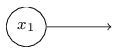
\includegraphics[scale=0.5]{img12.png}
\end{figure}

Considérons un réseaux neuronal arbitraire comme celui-ci-dessous : 

%imagen
 \begin{figure}[H]
 \centering
    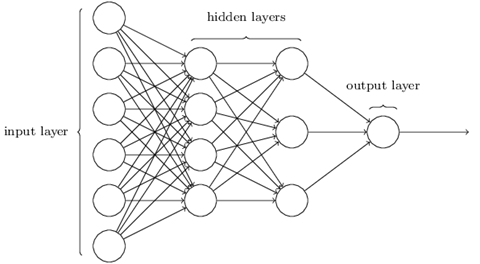
\includegraphics[scale=0.7]{img13.png}
\end{figure}


La colonne de gauche qui contient toutes les entrées est connue comme “couche d’entrée” (input layer en anglais). La colonne de droite qui contient toutes les sorties est connue comme “couche de sortie” (output layer en anglais). Les autres colonnes qui contiennent les neurones sont connues comme “couches cachés” (hidden layers en anglais). Dans le cas de l’image ci-dessus, on a un réseau neuronal avec 6 entrées (input features en anglais), 2 couches cachés et une sortie.  Il est important de remarquer que ce type de réseau neuronal, qui est composé d’une couche d’entrées, 2 couches cachées et une couche de sortie, est connue sous le nom de réseau neuronal pré-alimenté.
\hfill\\

\subsubsection{Réseau de neurones récurrents (Recurrent Neural Networks, RNN)}

Les réseaux de neurones récurrents sont un autre type de réseau de neurones. Il se caractérisent par le fait que la sortie donnée par une neurone est la sortie générale du réseau et au même temps, cette sortie est l’entrée pour le neurone suivante, comme l'ilustre l'image ci-dessous : 

%imagen
 \begin{figure}[H]
 \centering
    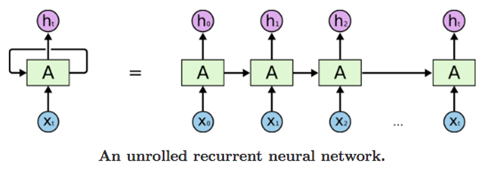
\includegraphics[scale=0.5]{img14.png}
\end{figure}


Le réseau de neurones récurrent est symbolisé comme le réseau de gauche avec une boucle de retro alimentation, cependant, il est plus de comprendre son fonctionnement en la “déroulant” (unroll en anglais) comme nous pouvons voire dans le réseau de neurones équivalent de droite. Dans ce cas, les neurones sont représentés par des rectangles en vert et la lettre $A$, les entrées sont représentées par des cercles bleus et la lettre $X$ avec un indice, et les sorties son représenté par des cercles violets et la lettre $h$ avec un indice. Il faut remarquer que dans ce cas la couche d’entrée correspond à la rangée qui contiens toutes les entrées en bleus, la couche de sortie correspond à la rangé supérieure qui contiens toutes les sorties en violet et la couche restante est la seule couche cachée. 

On observe que le neurone $A$, dans un premier temps, a comme entrée $X_0$. Elle réalise une fonction en fonction du type de neurone duquel elle fait partie et produit comme sortie la première sortie du réseau $h_0$.  Cette neurone fiat une retro alimentation avec la sortie qu’elle produit lorsque l’entrée est $X_1$ et ainsi de suite. Dans d’autres réseaux de neurones, les entrées sont indépendantes les unes avec les autres, mais dans le cas des réseaux de neurones récurrents toutes les entrées sont reliées avec les autres. 

C’est-à-dire qu'un réseau de neurones récurrents, contrairement à un réseau de neurones pré alimenté, peut utiliser l’état internet des neurones (mémoire) pour traiter des séquences d’entrées. Ceci explique pourquoi elles peuvent être utiliser pour des travaux comme la reconnaissance d’écriture ou vocale. 

La formule qui décret la sortie d’un réseau de neurones récurrent est la suivante :

\begin{equation}
    h_t = g(w_{t-1}h_{t-1} + w_tX_t) 
\end{equation}


Où g est la fonction d’activation du neurone.  

\subsubsection{Deep Learning}
Il s’agit d’une méthode de Machine Learning qui « apprend » aux ordinateurs à faire ce que nous, les être humain, arrivons à faire naturellement \textbf{apprentissage par exemples}. La plupart des méthodes de \textit{deep learning} utilisent des architectures de réseaux de neurones, c’est pour cette raison que la méthode de deep learning sont connue aussi sous le nom de \textit{deep learning networks}. Le therme « deep » fait référence au nombre de couches présentes dans les réseaux de neurones. En effet, les réseaux de neurones traditionnels ont entre 2 et 3 couches cachées, cependant les réseaux deep (deep networks) peuvent avoir beaucoup plus, par exemples elles peuvent contenir 150 couches cachées.
\medskip

Les modèles de deep learning s’entrainent en utilisant de grands ensembles de données étiquetées et des architectures de réseaux qui apprennent des caractéristiques directement des données sans besoin d’effectuer une extraction manuelle des caractéristiques en question. Cette dernière est la principale différence avec \textit{machine learning}, où l’extraction des caractéristiques remarquables se fait manuellement. Dans le cas du deep learning, ces caractéristiques sont extraites automatiquement , et en plus, il réalise un apprentissage « du début jusqu’à la fin » (\textit{end-to-end learning}), où un réseau reçoit les données brutes et à un revoir qui réalise, par exemple classifier, et apprend comment le faire automatiquement. L’image ci-dessous est un exemple de la différenciation entre machine learning et deep learning.

%imagen
 \begin{figure}[H]
 \centering
    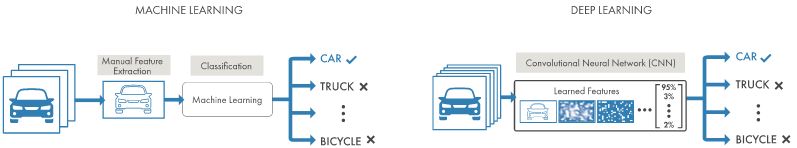
\includegraphics[scale=0.7]{DeepLearning.png}
    \caption{Comparaison d’un point de vue de machine learning pour catégoriser des véhicules (gauche) avec un de deep learning (droite).}
\end{figure}

\subsubsection{Algorithme du  Gradient}
\hfill\\
Il s’agit d’un algorithme d’optimisation qui est utilisé pour réduire le cout d’une fonction lorsque celle-ci se déplace itérativement dans la direction de la descente la plus importante selon ce qui est définie par le négatif du gradient. En machine learning, on l’utilise pour mettre à jour les paramètres du modèle. Les paramètres sont le poids des réseaux de neurones.
\href{https://ml-cheatsheet.readthedocs.io/en/latest/gradient_descent.html}{fuente}
\medskip

\subsubsection{The Vanishing Gradient Problem}
\hfill\\
Il s’agit d’entrainer les réseaux de neurones artificiels avec de méthodes d’apprentissage basé sur le gradient  et la rétropropagation du gradient (\textit{backpropagation}). Dans ces méthodes, chacun des poids du réseau de neurones reçoit une mise à jour proportionnel à la dérivée partielle de la fonction de l’erreur ou de cout par rapport au poids actuel en chaque itération de l’entrainement. Le problème est que dans certain cas, le gradient est tellement petit, qu’il prévient qu’un certain poids soit mis à jour ou change sa valeur. Dans le pire des cas, ceci arrivera totalement dans l’entrainement du réseau de neurones. 
\href{https://en.wikipedia.org/wiki/Vanishing_gradient_problem}{fuente}
\medskip


\subsubsection{\textbf{RNNbruit: Méthode hybride DSP/Deep Learning}}
\medskip
\hfill
\medskip

Después de haber aclarado los conceptos anteriores, resulta más simple la discusión del método y cómo los involucra. En primer lugar, la \textbf{supresión de ruido} es un tema viejo en el campo de procesamiento de voz (\textit{speech processing}), \href{https://ieeexplore.ieee.org/document/1163209}{que data desde los 70's}, y que como el nombre lo indica la idea es simple: tomar una señal ruidosa y remover tanto ruido como sea posible causando mínima distorsión para el audio de voz de interés.

%imagen
 \begin{figure}[H]
 \centering
    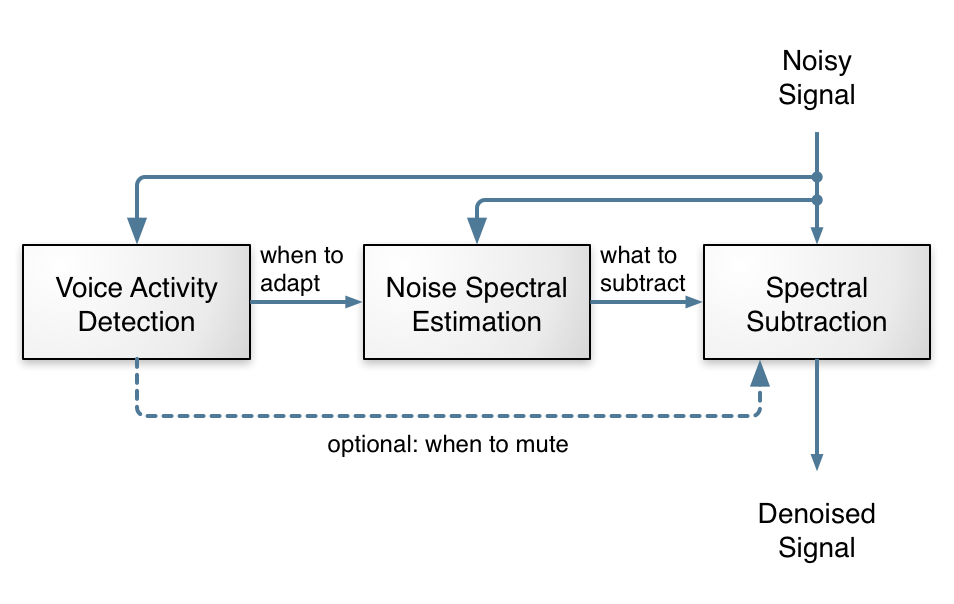
\includegraphics[scale=0.7]{noise_suppression.png}
    \caption{Esta es una visión conceptual de un algoritmo convencional de supresión de ruido. Un módulo de detección de actividad de voz o VAD (\textit{Voice Activity Detection}) detecta cuándo la señal contiene voz y cuándo es solo ruido. Esto es utilizado por un módulo de estimación espectral de ruido (\textit{Noise Spectral Estimation}) para descifrar las características espectrales del ruido(cuánta potencia hay en cada frecuencia). Luego, sabiendo cómo es el ruido, puede ser "substraído" (no es tan simple como suena) del audio de entrada}
    \label{Figure 14}
\end{figure}

El único problema de la imagen de arriba es que pareciera que la supresión de ruido es simple: hacer estas 3 tareas conceptuales y ya está. Esto no es del todo cierto, pues \underline{la parte
difícil} es hacer que el algoritmo funcione bien, todo el tiempo, para todos los tipos de ruido. Esto requiere que el algoritmo sea configurado meticulosa y cuidadosamente para cada caso particular, por lo que la opinión más común sobre el tema se resume en "50\% ciencia, 50\% arte".

Después de aclarar esto, viene la parte del \textbf{deep learning y las redes neuronales recurrentes}. El deep learning es la nueva versión de una idea vieja: redes neuronales artificiales. Aunque éstas han estado desde los 60s, lo que es nuevo en los años recientes es que:

\begin{enumerate}
    \item Ahora sabemos cómo hacerlas más profundas que 2 capas ocultas
    \item Ahora sabemos cómo hacer que las redes recurrentes recuerden patrones del pasado
    \item Ahora tenemos los recursos computacionales para entrenarlas
\end{enumerate}

Las redes neuronales recurrentes son muy importantes para el método porque hacen posible modelar secuencias de tiempo en vez de solo considerar entradas y salidas independientemente. Esto es especialmente importante para la supresión de ruido \underline{porque necesitamos tiempo para obtener un buen estimado del ruido}. Durante un tiempo las RNNs estaban altamente limitadas en su habilidad debido a dos problemas: no podían retener información por un largo periodo de tiempo y porque el proceso de gradiente descendente involucrado en la propagación hacia atrás (\textit{back-propagating}) a través del tiempo era muy ineficiente (problema de desvanecimiento de gradiente). Ambos problemas fueron solucionados por la invención de \textit{unidades cerradas} (\textit{gated units}), tales como las LSTMs (\textit{Long Short-Term Memory}), las GRUs (\textit{Gated Recurrent Unit}), y sus muchas variantes.


RNNbruit usa las unidades recurrentes cerradas (GRU) porque funcionan mejor que las LSTM en esta tarea y requieren menos recursos computacionales (CPU y memoria). Comparada con las unidades recurrentes simples, las GRUs tienen dos compuertas extra. La compuerta de reinicio (\textit{reset gate}) controla si el estado (memoria) es usado en la computación del nuevo estado, mientras que la compuerta de actualización (\textit{update gate}) controla cuánto cambiará el estado basado en la nueva entrada. Esta compuerta de actualización (cuando está apagada) hace posible (y mucho más fácil) para la GRU el poder recordar información por un largo periodo de tiempo y es la razón de que las GRUs (y las LSTMs) desempeñen mejor que unidades recurrentes simples.

%imagen
 \begin{figure}[H]
 \centering
    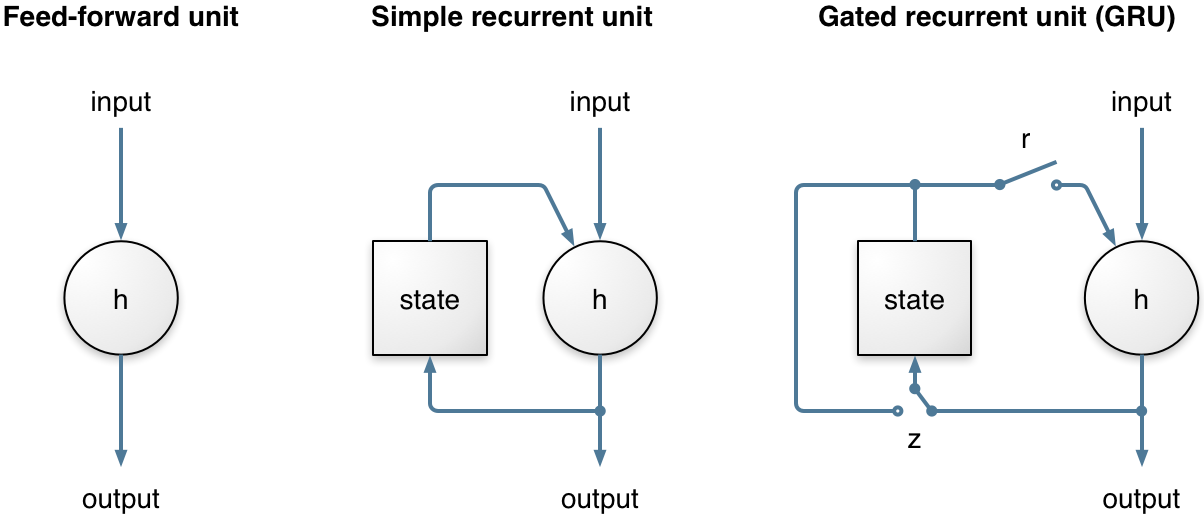
\includegraphics[scale=0.7]{simple_vs_gru.png}
    \caption{Comparación de una unidad simple recurrente con una GRU. La diferencia está en las compuertas $r$ y $z$ de la GRU, que hacen posible el aprendizaje de patrones a largo plazo. Ambas son suiches suaves (\textit{soft switches}, con valores entre 0 y 1) computados basados en el estado previo de toda la capa y las entradas, con una función de activación sigmoide. Cuando la compuerta de actualización $z$ está en la izquierda, entonces el estado puede permanecer constante sobre un largo periodo de tiempo $-$ hasta que una condición cause que la compuerta $z$ cambie a la derecha.} 
\end{figure}

Gracias al éxtio del deep learning, ya es popular "tirar" redes neuronales deep a un problema entero. Estos enfoque se le conoce como \textit{end-to-end} $-$ en donde son neuronas de principio a fin. Estos enfoques \textit{end-to-end} han sido aplicados a \href{https://arxiv.org/pdf/1412.5567.pdf}{reconocimiento de voz \textit{(speech recognition)}} y a \href{https://deepmind.com/blog/article/wavenet-generative-model-raw-audio}{síntesis de voz (\textit{speech synthesis})}. Por una parte, estos sistemas \textit{end-to-end} han probado qué tan poderosas pueden ser las redes neuronales deep. Por otra parte, estos sistemas pueden ser tanto suboptimales, y antiproducentes en términos de recursos. Por ejemplo, algunos enfoques de supresión de ruido usan miles de neuronas y deceneas de millónes de pesos (\textit{weights}) para realizar la supresión. El inconveniente no es solo el costo computacional, sino también el tamaño del propio modelo, donde se tienen miles de líneas de código y decenas de megabytes (o más) de pesos de neuronas.


Por esta razón el método RNNbruit utiliza un \textbf{enfoque híbrido}: mantener todo el procesamiento básico de señal que igual es necesario (no dejar que una red neuronal intente emularlo), pero dejar que la red neuronal aprenda todas las partes complicadas que requieren de configuración sin fin en paralelo al procesamiento de señal.

%imagen
 \begin{figure}[H]
 \centering
    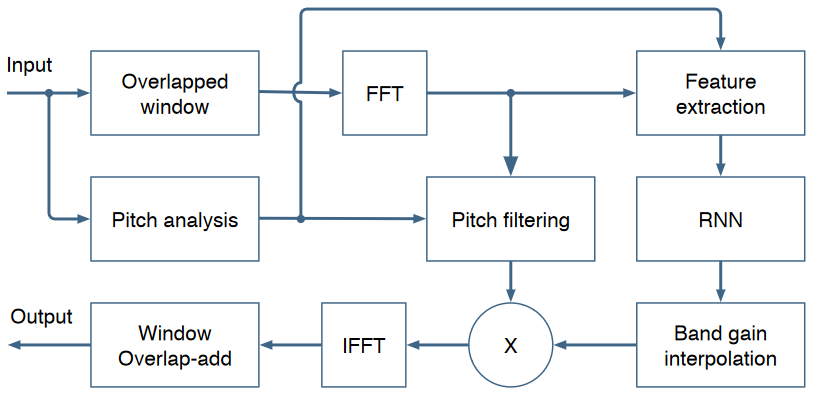
\includegraphics[scale=0.7]{Block_Diagram.png}
    \caption{Diagrama de bloques, en donde la red neuronal es representada por el bloque RNN y todo el enfoque deep corresponde a la columna más a la derecha, el resto hacen parte del procesamiento básico de señal. Esto evidencia el enfoque híbrido trabajando en paralelo.}
    \label{Figure 16}
\end{figure}

Otro aspecto diferente a algunos de los trabajos existentes de supresión de ruido con deep learning es que se apunta a la comunicación en tiempo real en vez del reconocimiento de voz, por lo que no se puede permitir mirar hacia adelante más que unos pocos milisegundos (en este caso $10 ms$).
\medskip

\paragraph{\textbf{Definición del problema}}
\hfill\\
\hfill

Para evitar tener un gran número de salidas $-$ y por lo tanto, un gran número de neuronas $-$ el método se diseñó para que no trabajara directamente con muestras (\textit{samples}) o con un espectro. En cambio, se consideran \textit{bandas} (\textit{bands}) de frecuencia que siguen la escala de Bark, una escala de frecuencia que coincide con cómo percibimos los sonidos. Logrando así usar un total de 22 bandas, en vez de 480 valores espectrales (complejos) que se hubieran tenido que considerar.

%imagen
 \begin{figure}[H]
 \centering
    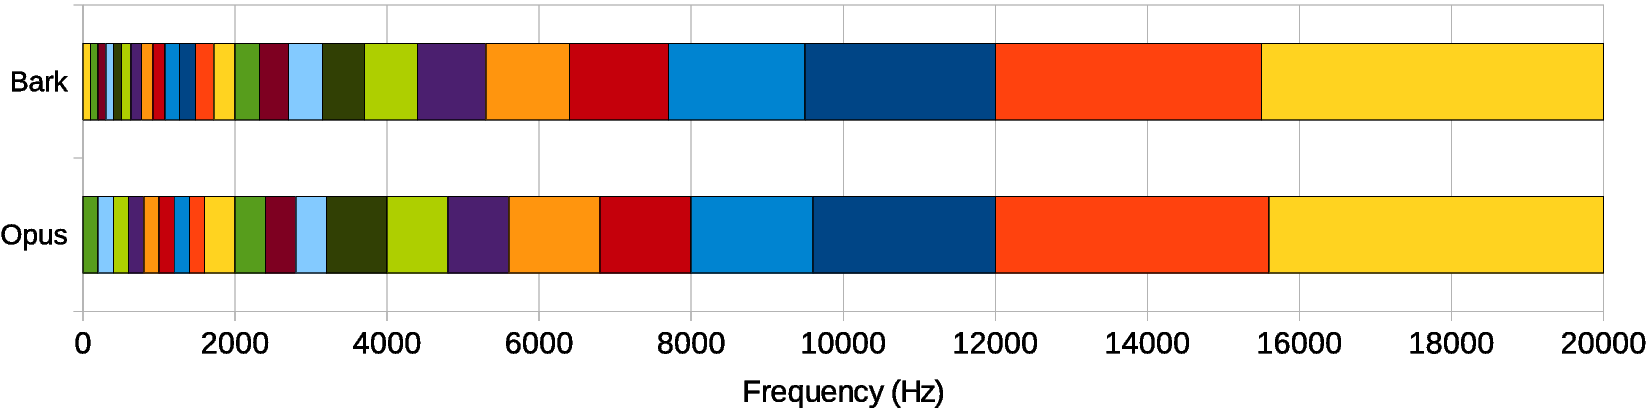
\includegraphics[scale=0.25]{bands.png}
    \caption{Comparación de las bandas Opus vs la escala de Bark actual. Para RNNbruit, se usa Opus como base. Dado que se superponen las bandas, los límites entre las bandas de Opus se convierten en el centro de las bandas superpuestas de RNNbruit. Las bandas son más anchas a alta frecuencia porque el oido tiene menor resolución de frecuencia ahí. A bajas frecuencias, las bandas son más estrechas, pero no tan anchas como las de la escala de Bark porque entonces no se tendrían suficientes datos para hacer buenos estimados.} 
\end{figure}

Es claro que no se puede reconstruir un audio tan solo usando 22 bandas de energía. Pero lo que sí se puede hacer es computar una ganancia que aplicar a la señal para cada una de esas bandas. Una forma simple de imaginarlo es pensar en usar un ecualizador de 22 bandas y rápidamente cambiar el nivel o volumen para cada banda para que atenuar el ruido, pero dejar pasar la señal.

%imagen
 \begin{figure}[H]
 \centering
    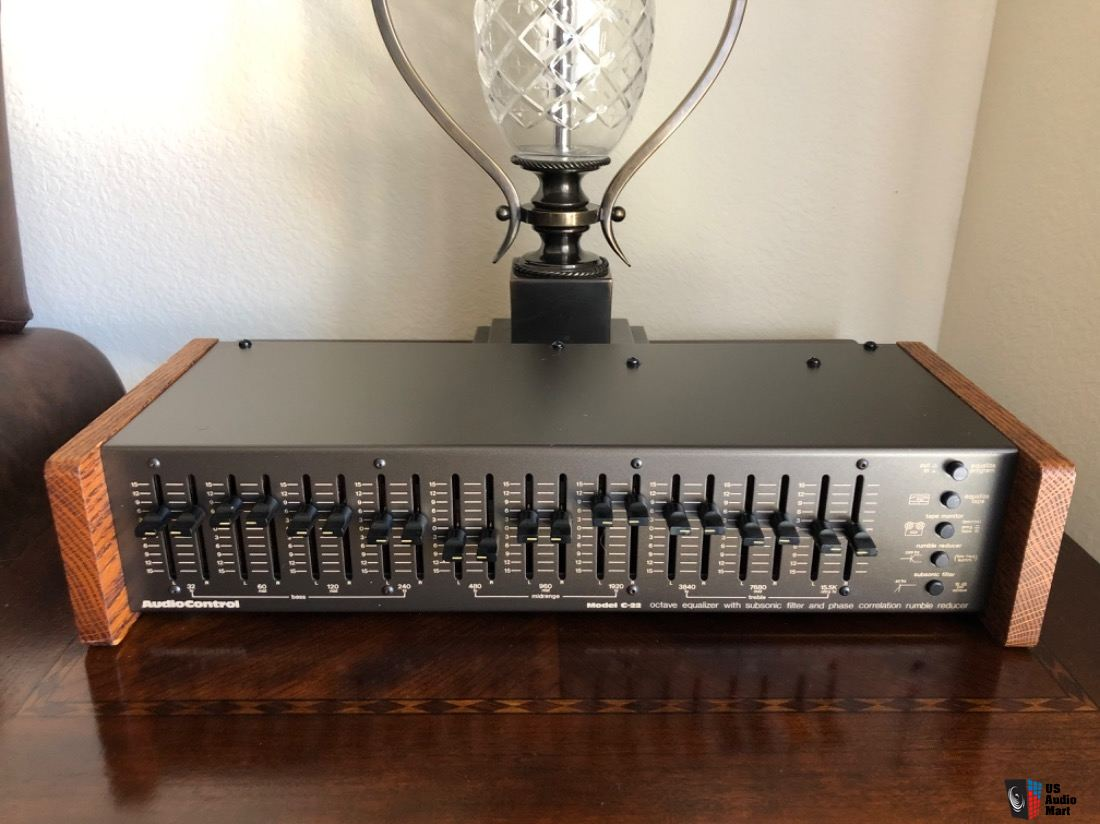
\includegraphics[scale=0.2]{22bEq.jpg}
    \caption{Ecualizador gráfico vintage \href{https://www.canuckaudiomart.com/details/649586296-vintage-audio-control-c-22-octave-10-band-equalizer/images/2554905/}{AudioControl C-22}. Cada uno de los botones verticales que suben y bajan (\textit{faders}) representan el volumen de una frecuencia en particular; RNNbruit funciona de forma similar.} 
\end{figure}

Hay varias ventajas de trabajar con ganancias por banda:
\begin{enumerate}
    \item Se obtiene un modelo más simple porque se computan menos bandas.
    \item Se hace imposible crear los llamados \href{https://www.vocal.com/noise-reduction/musical-noise/}{"artefactos de ruido musical" (\textit{musical noise artifacts})}, donde únicamente un tono logra pasar mientras sus "vecinos" son atenuados. Estos artefactos son comunes en la supresión de ruido y son bastante molestos. Con bandas suficientemente anchas, se deja pasar toda la banda completa o se corta por completo.
    \item La optimización del modelo. Como las ganancias de las bandas siempre están acotadas entre $0$ y $1$, simplemente usar una función de activación sigmoide (cuya salida también está entre $0$ y $1$) para computarlas garantiza que nunca se puede hacer algo realmente estúpido, como agregar ruido que no estaba ahí en primer lugar.
\end{enumerate}

La desventaja principal de la menor resolución que se obtiene al usar bandas es que no se tiene un resolución lo suficientemente fina como para suprimir el ruido entre los armónicos de tono (\textit{pitch harmonics}). Afortunadamente, no es tan importante y se logra con procesamiento de señal básico tal y como se muestra en el módulo \textit{Pitch filtering} en \ref{Figure 16}.

\medskip
\paragraph{\textbf{Arquitectura deep}}
\hfill\\
Como la salida que se computa se basa en 22 bandas, no tiene sentido tener mayor frecuencia de resolución en la entrada, entonces se utilizan las mismas 22 bandas para enviar enviar la información espectral a la red neuronal. Debido a que \href{https://www.britannica.com/science/dynamic-range}{el audio tiene un gran rango dinámico}, es mejor computar el $log$ de la energía en vez de enviar la energía directamente a la red. Se usa un proceso de decorrelación (\textit{decorrelate}) de las características usando una \href{https://dsp.stackexchange.com/questions/27810/how-to-understand-the-de-correlation-property-of-dct-what-does-de-correlation-m}{transformada discreta de coseno (DCT, \textit{Discrete Cosine Transform})}. Resultando en un \href{https://es.wikipedia.org/wiki/Cepstrum}{\textit{cepstrum}} basado en la escala de Bark, el cual está altamente relacionado con los Coeficientes Cepstrales de Frecuencia-Mel (MFCC, \href{https://en.wikipedia.org/wiki/Mel-frequency_cepstrum}{\textit{Mel-Frequency Cepstral Coefficients})} que son comunmente usados en reconocimiento de voz.


En adición a los coeficientes, RNNbruit también incluye:

\begin{itemize}
    \item La primera y segunda derivada de los primeros 6 coeficientes \textbf{(12 características de entrada)}
    \item El periodo del tono ($1$/$frecuencia fundamental$) \textbf{(1 característica de entrada)}
    \item La ganancia del tono (\textit{voicing strength}) en 6 bandas \textbf{(6 características de entrada)}
    \item Un valor especial para detección de voz \textbf{(1 característica de entrada)}
\end{itemize}

\hfill\\
Lo que quiere decir que RNNbruit usa en total 42 características de entrada a la red neuronal recurrente, lo cual se observa en la imagen a continuación.

%imagen
 \begin{figure}[H]
 \centering
    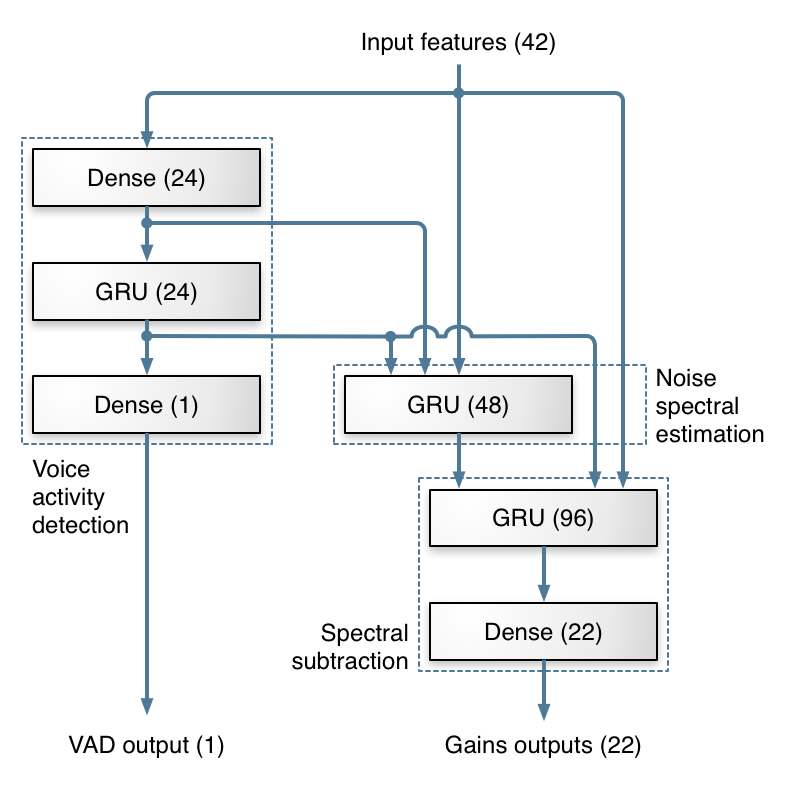
\includegraphics[scale=0.7]{topology.png}
    \caption{Topología de la red neuronal que usa RNNbruit. Cada caja representa una capa de neuronas, con el número de unidades indicado en paréntesis. Las capas densas (\textit{Dense}) son capas no recurrentes, mientras que claramente, las GRU sí lo son. Una de las salidas de la red es un conjunto de ganancias que aplicar a las 22 bandas de frecuencias (\textit{Gains outputs (22)}). La otra salida es la probabilidad de activación \textit{VAD output(1)}), que no se utiliza en la supresión de ruido pero que es un subproducto útil de la red.} 
\end{figure}

La arquitectura deep usada está inspirada en el enfoque tradicional de supresión de ruido como el que se muestra en \ref{Figure 14}. Note que en este caso cada uno de los 3 módulos usa redes neuronales y se muestran enmarcados en líneas azules punteadas. La mayoría del trabajo es realizado por las 3 capas de GRU. Cabe resaltar que, por supuesto, así como usualmente es el caso con las redes neuronales no se tienen pruebas de que la red está usando las capas de la forma en la que se pretende, pero el hecho de que la topología funcione mejor que otras intentadas por los creadores del método, hace que sea razonable pensar que se comporta como fue diseñado.

\paragraph{\textbf{Código e implementación}}
El código del método es de libre acceso y se encuentra disponible en el repositorio de GitHub \href{https://github.com/xiph/rnnoise}{xiph/rnnoise}. Todo el diseño y entrenamiento de la red neuronal es realizado en Python usando la libreria de deep learning \href{https://keras.io/}{Keras}, pero todo el código de ejecución es realizado en C bajo una \href{https://es.wikipedia.org/wiki/Licencia_BSD}{licencia BSD} un tipo de sistema operativo tipo Unix.

El sistema operativo escogido para esta labor fue \href{https://ubuntu.com/download/desktop}{Ubuntu 20.04.1} un sistema operativo (64-bit) open source. Sin embargo, debido a que este no es el sistema operativo de preferencia personal se decidió utilizar una máquina virtual usando el software \href{https://www.virtualbox.org/}{Oracle VirtualBox 6.1} (otro software open source) utilizando como sistema operativo principal o \textit{host} Microsoft Windows 10 Home Single Language. A continuación se muestra una imagen de la máquina virtual junto con las características seleccionadas. Note que entre las características se muestra que hay una carpeta compartida entre el \textit{host} y la máquina virtual. Esto para facilitar los archivos de entrada y salida del método.

%imagen
 \begin{figure}[H]
 \centering
    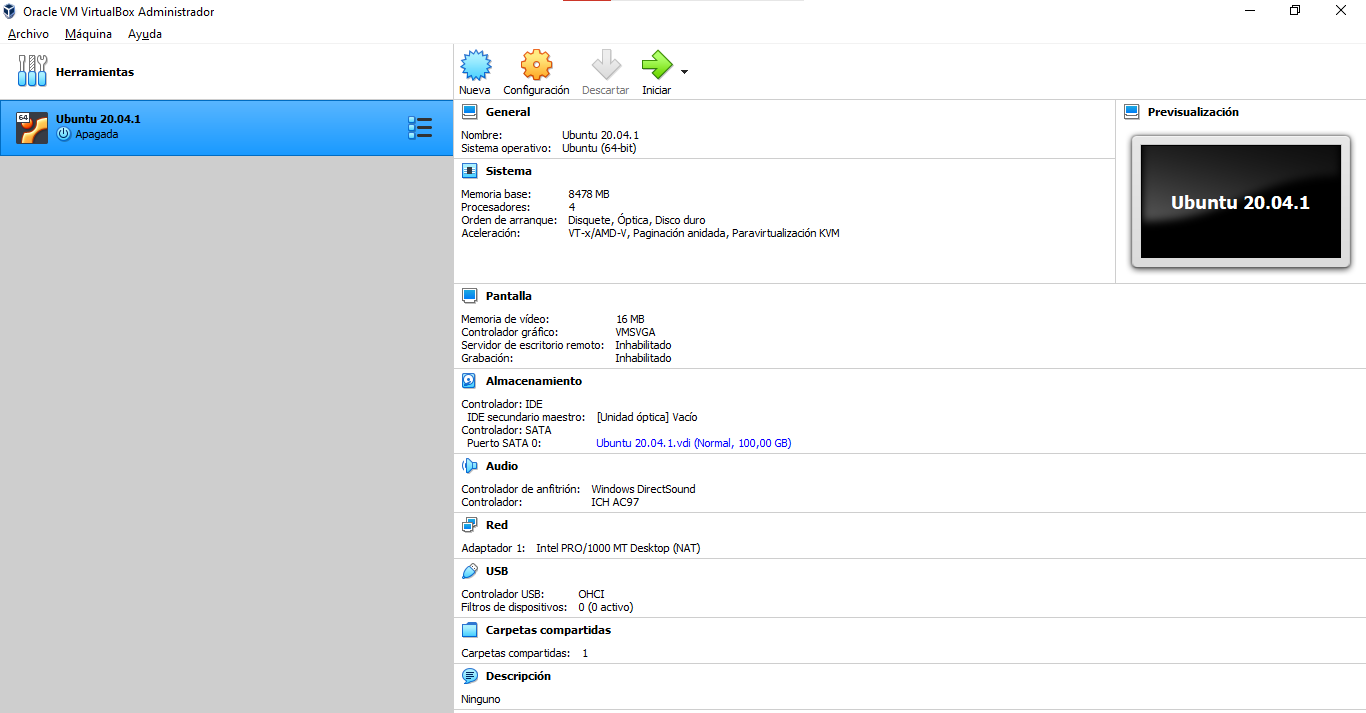
\includegraphics[scale=0.45]{VM1.png}
    \caption{Características de la máquina virtual de Ubuntu implementada} 
\end{figure}

A continuación se muestra una captura de pantalla del funcionamiento de la máquina virtual.

%imagen
 \begin{figure}[H]
 \centering
    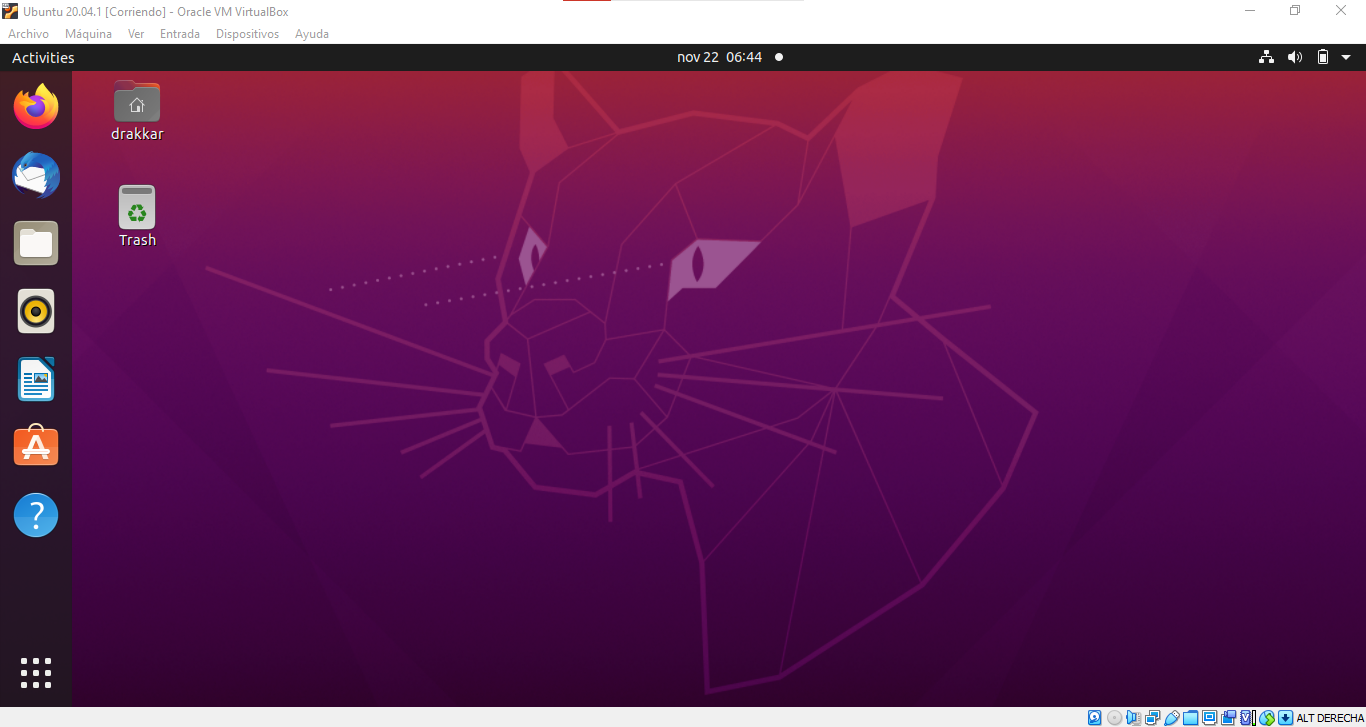
\includegraphics[scale=0.45]{VM2.png}
    \caption{Máquina virtual encendida} 
\end{figure}
\hfill\\
Luego de descargar el código del repositorio mencionado anteriormente, se siguieron las instrucciones del \texttt{README} disponible allí, con el fin de "activar" el método. Las instrucciones se muestran a continuación.

%imagen
 \begin{figure}[H]
 \centering
    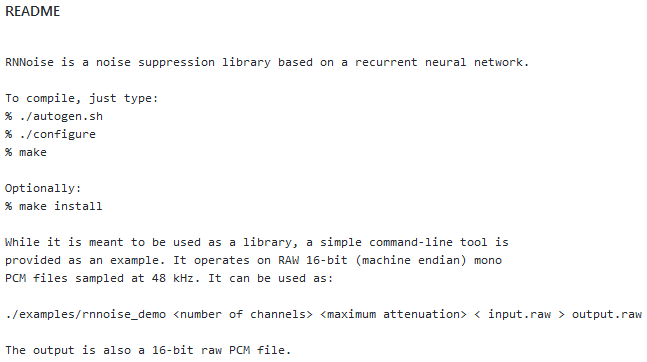
\includegraphics[scale=0.7]{VM3.png}
    \caption{Instrucciones para activar o compilar el método RNNbruit} 
\end{figure}

Siguiendo las instrucciones se muestra un ejemplo de la ejecución del método RNNbruit usando como ejemplo el audio de entrada \texttt{AW0,3.wav} y especificando el nombre del audio de salida como \texttt{SALIDA.wav}.

%imagen
 \begin{figure}[H]
 \centering
    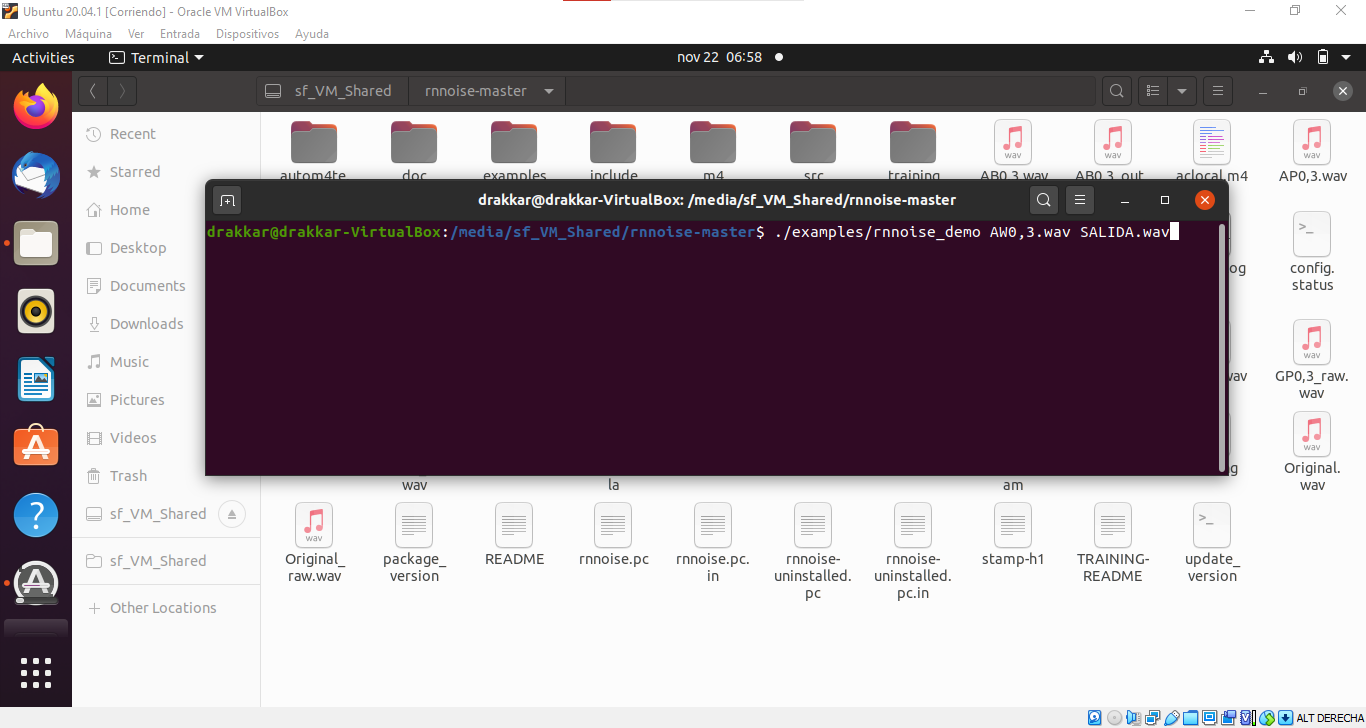
\includegraphics[scale=0.45]{VM4.png}
    \caption{Ejecución del método RNNbruit} 
\end{figure}
\hfill\\

Observe en la imagen a continuación que la ejecución del método se realizó exitosamente y el archivo \texttt{SALIDA.wav} fue creado.

%imagen
 \begin{figure}[H]
 \centering
    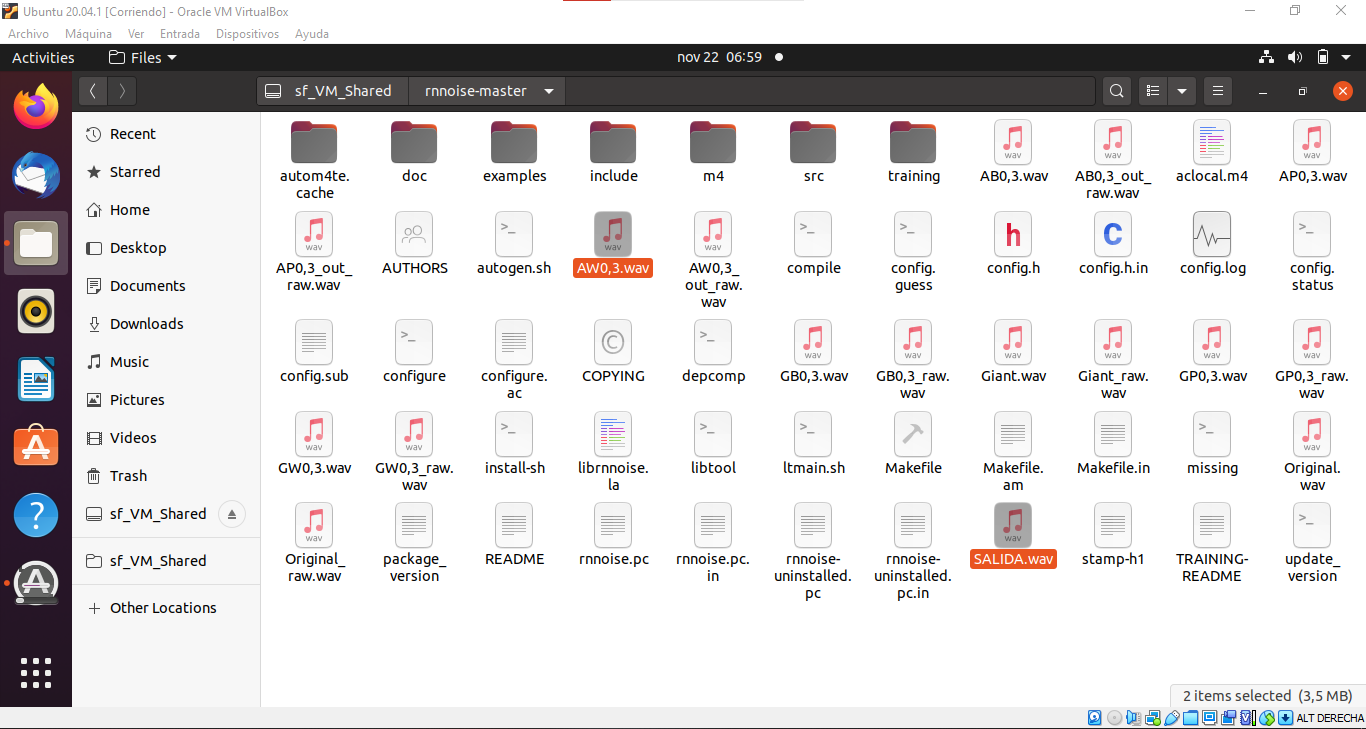
\includegraphics[scale=0.4]{VM5.png}
    \caption{Audio de entrada y audio de salida resultante.} 
\end{figure}

Aunque el audio resultante aunque esté almacenado en formato \texttt{.wav} las instrucciones del método especifican que en realidad se está almacenando un archivo tipo \texttt{RAW PCM 16-bit}, por lo que si se intenta abrir o reproducir se produce un error. Observe este comportamiento a continuación.

%imagen
 \begin{figure}[H]
 \centering
    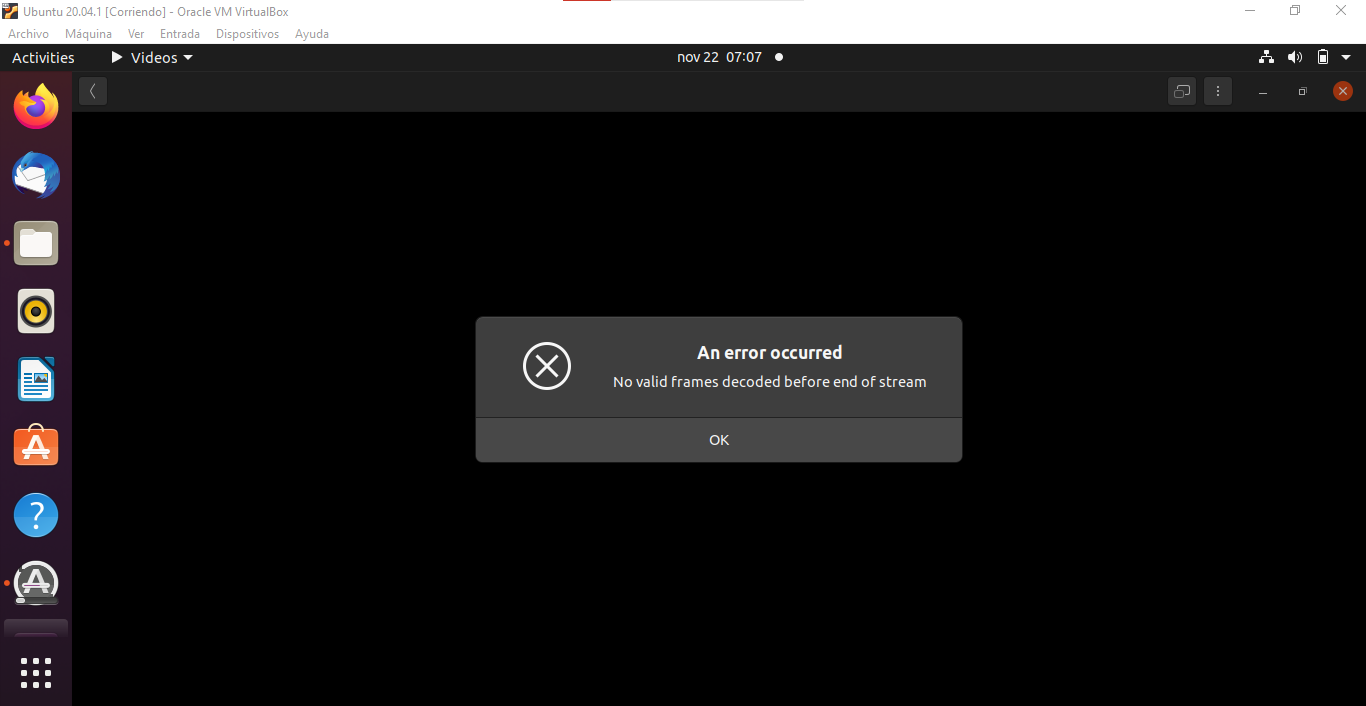
\includegraphics[scale=0.4]{VM6.png}
    \caption{Error obtenido al intentar reproducir el audio de salida} 
\end{figure}

Para corregir el formato del audio de salida, se regresa al sistema operativo \textit{host}, se utiliza el software open source \href{https://www.audacityteam.org/}{Audacity 2.4.2} y se toma el archivo de la carpeta compartida con la máquina virtual. Para abrirlo de forma adecuada en Audacity se usan las opciones \texttt{File/import/Raw Data...} tal y como se muestra a continuación.

%imagen
 \begin{figure}[H]
 \centering
    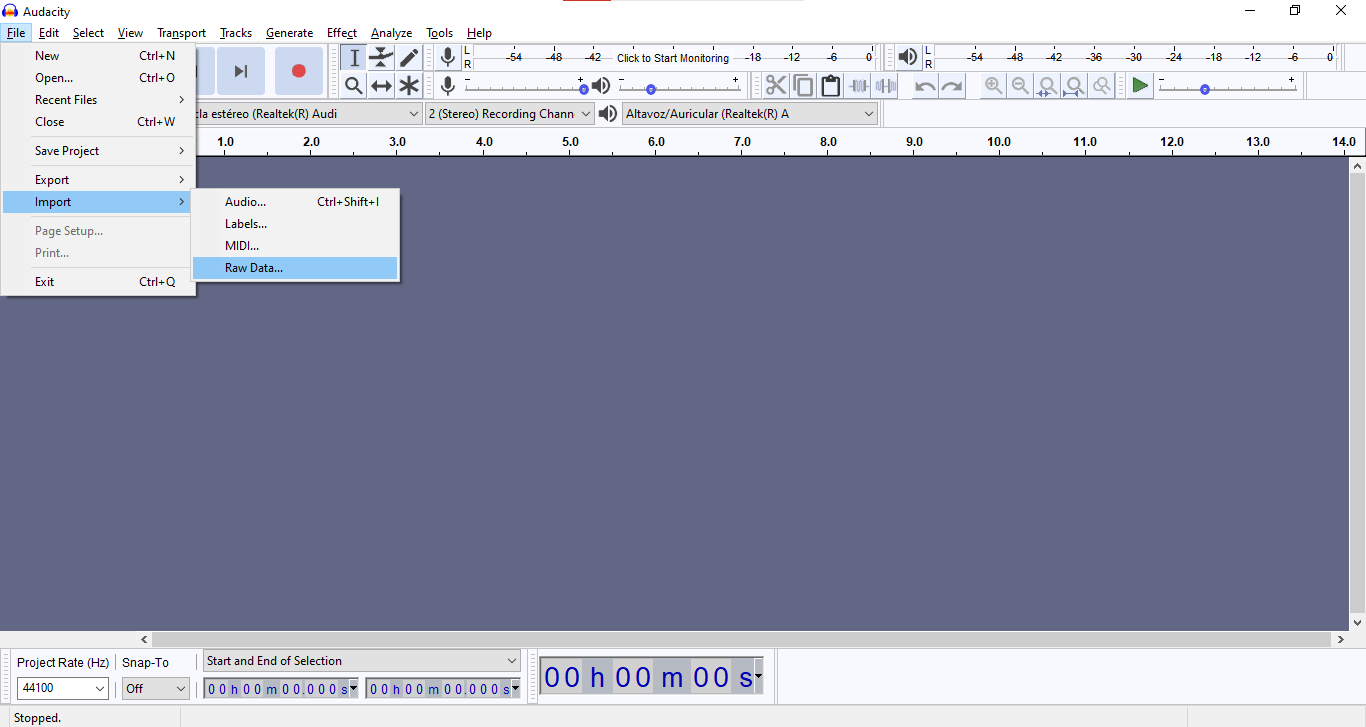
\includegraphics[scale=0.45]{VM7.png}
    \caption{Import del audio de salida en Audacity}
\end{figure}

Se selecciona el archivo de la carpeta compartida.

%imagen
 \begin{figure}[H]
 \centering
    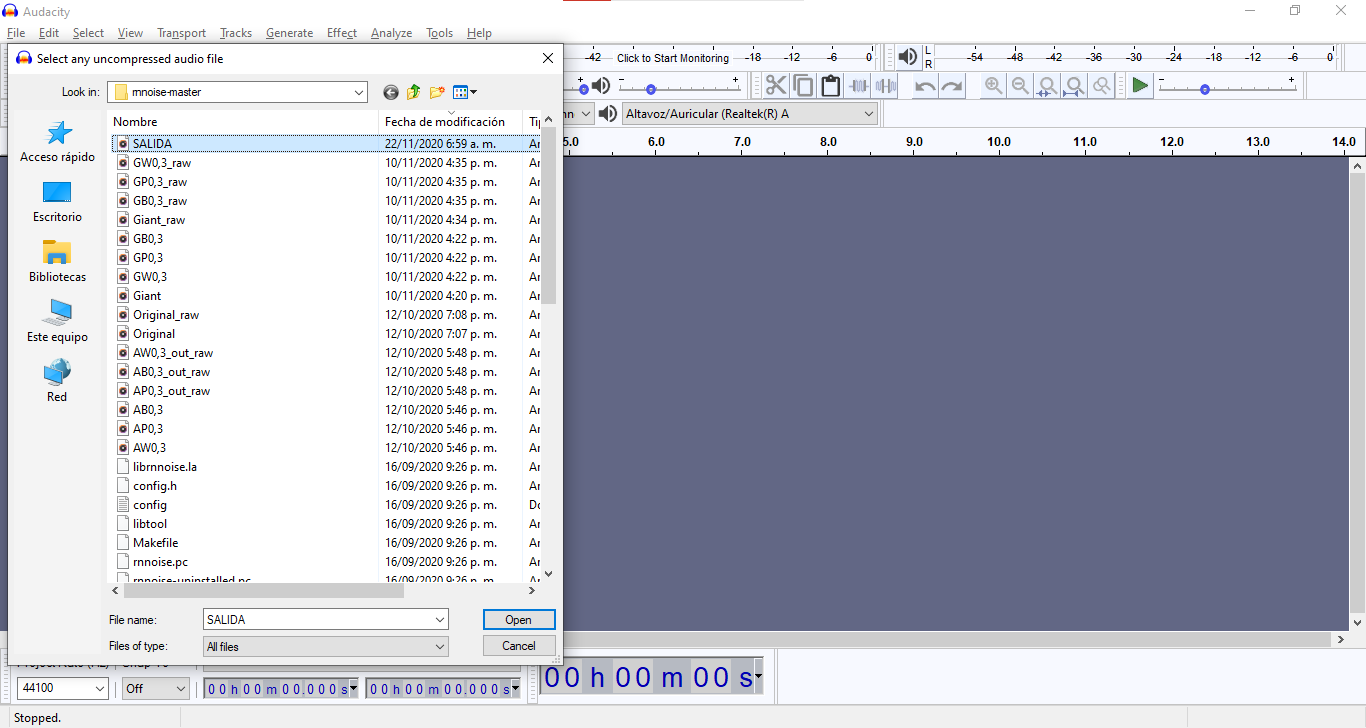
\includegraphics[scale=0.45]{VM8.png}
\end{figure}

Y se importa con las respectivas configuraciones.

%imagen
 \begin{figure}[H]
 \centering
    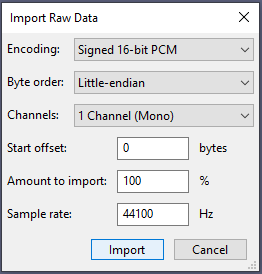
\includegraphics[scale=0.6]{VM9.png}
\end{figure}

Importando exitosamente el audio de forma reproducible en Audacity.

%imagen
 \begin{figure}[H]
 \centering
    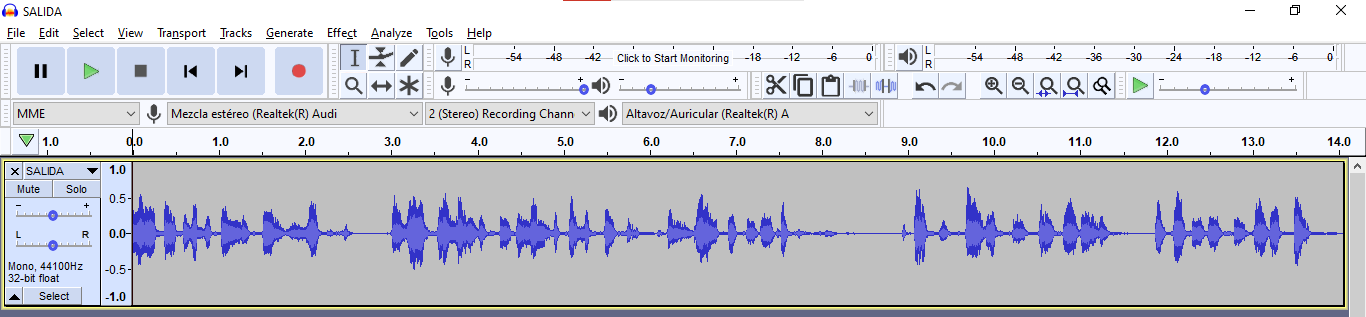
\includegraphics[scale=0.4]{VM10.png}
\end{figure}

El cual puede ser exportado correctamente simplemente al seguir las opciones \texttt{File/Export/Export as WAV} como se muestra a continuación.

%imagen
 \begin{figure}[H]
 \centering
    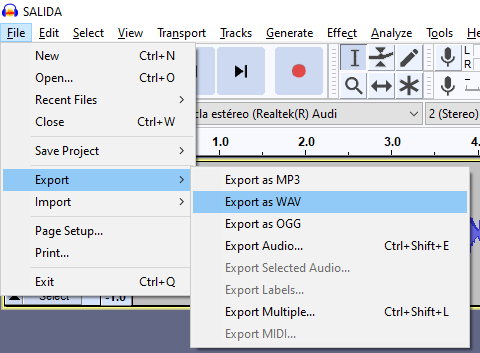
\includegraphics[scale=0.4]{VM11.png}
\end{figure}

Generando satisfactoriamente el audio de salida de forma reproducible.

%imagen
 \begin{figure}[H]
 \centering
    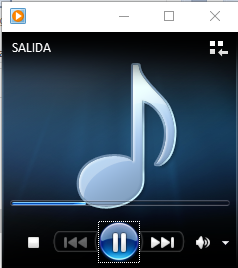
\includegraphics[scale=0.5]{VM12.png}
\end{figure}

\newpage
\section{Résultats et comparaison des méthodes}
Les méthodes ont été implémenter de manière qualitative et quantitative. Pour chaque cas, on a utilisé le software Matlab R2020a sur le SO Microsoft Windows 10 Home Single Language (v.10.0.19041). Pour les cas de l’implémentation a génère du bruit blanc, du bruit rose et du bruit rouge en utilisant le software Audicity 2.4.2. Après, sur Matlab on a pris l’enregistrement audio original et on a créé, à partir de ce dernier, 3 autres enregistrements audios en ajoutant 30\% du bruit blanc, 30\% du bruit rose et 30\% du bruit rouge, respectivement.

\subsection{Résultats quantitatifs}
Dans le tableau \ref{table:t1} on peut voir le pourcentage de bruit résultant lorsqu’on ajoute 30\% de bruit blanc a l’enregistrement audio et on le filtre avec chaque méthode.
\begin{table}[hbt!]
    \centering
    \begin{tabular}{ l  c }
    \textbf{Méthodes} & \textbf{Blanc (30\%)} \\
    \hline
    Sans méthode & 80.658 \\
    Wienner & 44.218 \\
    Butter T & 10 \\
    RNNbruit & 9.9668 \\
    \end{tabular}
    \caption{Résultats des méthodes pour 30\% du bruit blanc}
    \label{table:t1}
\end{table}
\hfill \\
Dans le tableau \ref{table:t2} on peut voir le pourcentage de bruit résultant lorsqu’on ajoute 30\% de bruit rose a l’enregistrement audio et on le filtre avec chaque méthode.
\begin{table}[hbt!]
    \centering
    \begin{tabular}{ l  c }
    \textbf{Méthodes} & \textbf{Rose (30\%)} \\
    \hline
    Sans méthode & 39.442 \\
    Wienner & 44.082 \\
    Butter T & 35 \\
    RNNbruit & 11.493 \\
    \end{tabular}
    \caption{Résultats des méthodes pour 30\% du bruit rose}
    \label{table:t2}
\end{table}
\hfill \\
Dans le tableau \ref{table:t3} on peut voir le pourcentage de bruit résultant lorsqu’on ajoute 30\% de bruit rouge a l’enregistrement audio et on le filtre avec chaque méthode.
\begin{table}[hbt!]
    \centering
    \begin{tabular}{ l  c }
    \textbf{Méthodes} & \textbf{Marron (30\%)} \\
    \hline
    Sans méthode & 53.969 \\
    Wienner & 36.209 \\
    Butter T & 35 \\
    RNNbruit & 7.7496 \\
    \end{tabular}
    \caption{Résultats des méthodes pour 30\% du bruit Marron}
    \label{table:t3}
\end{table}
\hfill \\

Premièrement, en étudiant les résultats obtenus par l'implémentation du filtre passe-bas avec une approximation de Butter Worth, nous confirmant les hypothèses théoriques vues précédemment. En effet, compte tenu que l’approximation de Butter Worth permet d’avoir une précision en amplitude. Cette précision est centre sur des bases fréquences. Nous voyons cela évidence dans le filtrage des bruits ajouter à notre signal. Lorsque nous ajoutons du bruit blanc et nous filtrons le signal résultant, nous constatons une diminution du pourcentage du bruit présent dans le signal. Alors que lorsque nous effectuons le même procédé pour le bruit rose et le bruit marron, le pourcentage de bruit ne change pas. Donc cette méthode avec cette approximation particulière est bien plus convenable pour filtrer le bruit blanc présent dans les enregistrements audios.

Dans un deuxième temps, le cas de la méthode hybride du RNNbruit, nous observons que cette méthode est belle et bien convenable pour les différents types de bruit additionnés. En effet, nous constatons une atténuation du bruit considérable dans chacun des cas. De plus, nous remarquons que cette méthode ne gêne pas la transmission du signal sonore, en d'autre thermes cette méthode lise et "purifie" le signal orignal. Nous pouvons expliquer ce comportement par la nature adaptative de la méthode, dû au fait de l'implémentation de réseau de neurones récurrents pour faire face au bruit non harmonique. Cependant, la partie traditionnelle de cette méthode dite hybride se charge du bruit harmonique comme nous l'avant vue précédemment dans la partie théorique.

Finalement, lorsque nous analysons les résultats obtenus en utilisant le filtre adaptatif de Weiner, nous apercevons que cette méthode de filtrage numérique a des meilleurs résultats sur du bruit blanc. Or, en effectuant une analyse auditive, nous pourrions penser que ce filtrage est bien plus efficace avec le bruit marron ou le bruit rose, nous pouvions affirmer théoriquement que ‘est avec le bruit blanc qu’il est plus efficace. En effet, en employant cette méthode nous introduisons des nouveaux types de bruits que nous ne considérerons pas dans notre analyse. Par exemple, dans le filtrage de l’enregistrement audio avec du bruit marron, nous pouvons avoir l’impression que le résultat est nettement plus compressible qu’avec du bruit blanc. Cependant, en regardant les résultats de l’analyse nous nous rends compte que l’audio résultant a perdu de l’intensité sonores, c’est-à-dire que l’amplitude de son gain en fréquence a considérablement diminuer. Cette méthode, théoriquement parlant, nous est convenable dans la mesure ou elle permet un filtrage du bruit blanc, mais elle rencontre ses limites avec les 2 autres types de bruit étudiés.


\subsection{Résultats qualitatifs}
\hfill \\
Dans le tableau \ref{table:t4} On peut voir la classifications que nous avons donné au résultat de chaque méthode de filtrage suite a un ajout de 30\% de bruit blanc au signal original. Cette classification va de 1 jusqu'á 10, où 1 signifie que la perception auditive est de très mauvaise qualité et 10 signifie que la perception auditive est de haute qualité.
\begin{table}[hbt!]
    \centering
    \begin{tabular}{ l  c }
    \textbf{Méthodes} & \textbf{Blanc (30\%)} \\
    \hline
    Wienner &  4\\
    Butter T &  8 \\
    RNNbruit &  8.5 \\
    \end{tabular}
    \caption{Qualification des méthodes pour 30\% du bruit blanc}
    \label{table:t4}
\end{table}
\hfill \\
Dans le tableau \ref{table:t5} On peut voir la classifications que nous avons donné au résultat de chaque méthode de filtrage suite a un ajout de 30\% de bruit rose au signal original. Cette classification va de 1 jusqu'á 10, où 1 signifie que la perception auditive est de très mauvaise qualité et 10 signifie que la perception auditive est de haute qualité.  
\begin{table}[hbt!]
    \centering
    \begin{tabular}{ l  c }
    \textbf{Méthodes} & \textbf{Rose (30\%)} \\
    \hline
    Wienner & 5 \\
    Butter T &  6 \\
    RNNbruit &  8 \\
    \end{tabular}
    \caption{Qualification des méthodes pour 30\% du bruit rose}
    \label{table:t5}
\end{table}
\hfill \\
Dans le tableau \ref{table:t6} On peut voir la classifications que nous avons donné au résultat de chaque méthode de filtrage suite a un ajout de 30\% de bruit rouge au signal original. Cette classification va de 1 jusqu'á 10, où 1 signifie que la perception auditive est de très mauvaise qualité et 10 signifie que la perception auditive est de haute qualité.
\begin{table}[hbt!]
    \centering
    \begin{tabular}{ l  c }
    \textbf{Méthodes} & \textbf{Marron (30\%)} \\
    \hline
    Wienner & 6  \\
    Butter T &  4.5 \\
    RNNbruit & 8 \\
    \end{tabular}
    \caption{Qualification des méthodes pour 30\% du bruit Marron}
    \label{table:t6}
\end{table}
\hfill \\


\newpage

\section{Méthodes modifiées}
En esta sección se realizan las descripciones e implementaciones de las modificaciones propuestas para cada uno de los métodos.

\subsection{\textbf{Butterworth modifiée}}

\subsubsection{Modifications de la fonction Matlab butter}

fonction Dans un premier temps, nous avons choisis de de faire une modification de la méthode Matlab Butter, méthode que nous utilisons pour la création du filtre passe-bas avec un approximation de Butterworth. Pour cela, nous avons ouvert la méthode ou plutôt de script de la fonction butter avec la ligne de code suivante :

\[ \texttt{edit butter}\]

Lorsque nous rentrant cette ligne de code, Matlab nous renvois le script de la fonction butter, ci-dessous vous trouverais 2 images correspondantes à 2 parties différentes de ce script. La première montre le début du code, c'est à dire les commentaires qui explique le code et ce qu'il fait. La deuxième partie correspond à la partie du code qui permet faire le choix du type de filtre que nous voulant créer (passe-bas, passe-haut, coupe-bande et réjecteur de bande).

%imagen
%buttermod1
 \begin{figure}[H]
 \centering
    \includegraphics[scale=0.3]{b1.jpeg}
\end{figure}


%imagen
%buttermod2
 \begin{figure}[H]
 \centering
    \includegraphics[scale=0.3]{b2.jpeg}
\end{figure}


Ensuite, nous avons cherché a modifié cette méthode sur les parties concernant les filtres passe bas. Il faut se rappeler que les filtres de butterworth sont de l’ordre n, ceci est la raison de notre modification. Nous voulons modifier l’ordre du filtre pour voir si cette modification entraine un changement dans les signaux de sortie obtenues. Pour cela, nous changeant l’ordre n des filtres passe bas de butterworth pour l’ordre 2n + 1. L’image ci-dessous montre une des modifications que nous avons fait dans le code.

%imagen
%buttermod3
 \begin{figure}[H]
 \centering
    \includegraphics[scale=0.3]{b3.jpeg}
\end{figure}


Après avoir effectué ces modifications nous procédons à sauvegarder les modifications, c'est à dire à sauvegarder le script butter.m sur lequel nous avons travaillé. Or, lorsque nous cliquons sur le buton "save" de Matlab, le message suivant nous apparait :

%imagen
%buttermod4
 \begin{figure}[H]
 \centering
    \includegraphics[scale=0.3]{b4.jpeg}
\end{figure}


Ce message veut dire que la fonction Matlab butter à une certaine privacité ce qui empêche toute modification de celle-ci. Par suite de cette découverte nous décidons d’effectuer la modification de la méthode en jouant avec la fréquence de coupure de celle-ci qui peut être considéré comme un paramètre externe de la fonction.

\subsubsection{Modification du filtre de Butterworth à partir de la fréquence}
Dans un deuxième temps, nous décidons d'effectuer la modification du filtre de passe-bas avec une approximation de Butterworth en jouant avec la fréquence de coupure. Tout d'abord, nous créant le filtre avec l'outil sptool de Matlab en rentrant la ligne de code ci-dessous :

\[\texttt{sptool}\]

Après avoir rentrée cette ligne de code une fenêtre dédier à l'analyse de signaux et création de filtres s'ouvre. En effet, sptool est un outil qui permet l'analyse des signaux, il est composé de 4 autres outils : Signal Browser, Filter Design and Analysis Tool, FVTool et Spectrum Viewer. Ces outils permettent l'accès a grande variété des fonctions des signaux, du filtrage et de l'analyse spectrale de la boite à outil. Lorsque nous rentrant dans ligne de code, elle exécute la commande SPTOOl.sptool et ouvre la fenêtre suivante :

%imagen
%buttermod5
 \begin{figure}[H]
 \centering
    \includegraphics[scale=0.3]{b5.jpeg}
\end{figure}


Nous allons nous intéresser aux colonnes Signals et Filters. Tout d'abords, la colonne Filters nous permet de créer un nouveau filtre. Pour cela, nous cliquons sur le buton New en bas de la colonne. En cliquant sur ce buton, une nouvelle fenêtre s'ouvre nous permettant de créer un nouveau filtre. Nous allons créer un filtre passe-bas de Butterworth d'ordre 2 avec une fréquence de coupure de 200 Hz et une fréquence de sortie de 60000 Hz. L'image ci-dessous illustre comment nous avons procédés pour créer le filtre en question.

%imagen
%buttermod6
 \begin{figure}[H]
 \centering
    \includegraphics[scale=0.3]{b6.jpeg}
\end{figure}


Premièrement dans l'onglet Reponse type nous choisissons le type de filtre que nous voulons, nous choisissons Lowpass pour dire que nous voulons un filtre passe-bas. Deuxièmement, dans l'onglet Desing Method nous choisissant la méthode que nous voulant, dans ce cas nous choisissons IIR Butterworth. Troisièmes dans l'onglet Filter Order, nous choisissons l'ordre du filtre, donc nous cochons l'option Specify Order et rentrant l'ordre que nous voulons étant un ordre 2. Finalement, nous rentrant la fréquence de sortie ($F_s$) et la fréquence de coupure ($F_c$) dans l'onglet Frequecy Specifications, et nous cliquons sur le buton Design Filter pour créer le filtre. 

Nous constatons aussi que lorsque notre filtre est créé nous pouvons voir le digramme de Bode de celui-ci, ainsi que son diagramme de phase et son gabarit. 

L'image ci-dessous correspond au diagramme de Bode du filtre de passe-bas de Butterworth modifier :

%imagen 
%buttermod7
 \begin{figure}[H]
 \centering
    \includegraphics[scale=0.3]{b7.jpeg}
\end{figure}


L'image ci-dessous correspond au diagramme de phase du filtre de passe-bas de Butterworth modifier :

%imagen 
%buttermod8
 \begin{figure}[H]
 \centering
    \includegraphics[scale=0.3]{b8.jpeg}
\end{figure}


L'image ci-dessous correspond au gabarit du filtre de passe-bas de Butterworth modifier :


%imagen 
%buttermod9
 \begin{figure}[H]
 \centering
    \includegraphics[scale=0.3]{b9.jpeg}
\end{figure}


Maintenant que nous avons notre filtre de Butterworth avec une nouvelle fréquence de coupure, nous procédons aux filtrages des signaux. Pour cette partie nous choisissons de filtrer $40s$ de la chanson \textit{« Giant »} de \textit{« Calvin Harris »} et \textit{Rag'n'Bone Man}, avec une addition de 30\% de bruit banc, rose et rouge.

Dans un premier temps, dans la ligne de code de Matlab, nous rentrant les lignes de codes suivantes :

\[ \texttt{[y,f]=audioread('Giant.wav')}\]
\[ \texttt{[yw,fw]=audioread('GW0,3.wav')}\]
\[ \texttt{[yp,fp]=audioread('GP0,3.wav')}\]
\[ \texttt{[yb,fb]=audioread('GB0,3.wav')}\]

Ces lignes de codes font appel à la fonction \texttt{audioread} de Matlab qui permet la lecture de fichier audio en format $.wav$. La première ligne de code permet donc la lecture de la chanson originale sans bruit ajouté, la deuxième lis la chanson avec un ajout de 30\% de bruit blanc, la troisième et quatrième font de même mais avec 30\% de bruit rosa et 30\% de bruit rouge respectivement.

Puis, nous revenons sur l'outil \texttt{sptool}, et nous importons les signaux. Pour cela nous allons sur l'onglet \texttt{File}, en haut à gauche, nous cliquons dessous et nous choisissons l'option \texttt{Import...}. Lorsque nous cliquons dessous une nouvelle fenêtre s'ouvre (voir image ci-dessous).

%imagen
%buttermod10
 \begin{figure}[H]
 \centering
    \includegraphics[scale=0.3]{b10.jpeg}
\end{figure}



Lorsque nous aurons effectué la lecture des signaux, la nouvelle fenêtre ressemblera à celle ci-dessous :

%imagen
%buttermod11
 \begin{figure}[H]
 \centering
    \includegraphics[scale=0.3]{b11.jpeg}
\end{figure}


Maintenant, nous choisissons un des signaux entre les suivants : y, yw, yp, yb. Et nous cliquons sur la petite flèche qui sépare la colonne \texttt{Workspace Contents} et \texttt{Import As:}. Tout en bas nous changeons le nom du signal, dans la colonne \texttt{Name} et nous écrivons le nom \texttt{Original} (voir image ci-dessous) et nous cliquons sur le buton \texttt{OK}.

%imagen
%buttermod12
 \begin{figure}[H]
 \centering
    \includegraphics[scale=0.3]{b12.jpeg}
\end{figure}


Notre signal a été importer. Si nous cliquons sur le buton \texttt{View} de la colonne \texttt{Signals} en choisissant notre signal, nous observerons le spectre en fréquence du signal, comme le montre l'image ci-dessous.

%imagen
%buttermod13
 \begin{figure}[H]
 \centering
    \includegraphics[scale=0.3]{b13.jpeg}
\end{figure}


Ensuite nous allons appliquer notre filtre à ce signal. Pour cela, nous cliquons sur notre signal, puis sur notre filtre et nous cliquons sur le buton \texttt{Apply}. Celui fera filtrer le signal original para notre filtre de Butterworth. Après avoir cliqué sur \texttt{Apply} une fenêtre apparait qui nous permet de changer le nom du signal de sortie, comme le nombre l'image suivante:

%imagen
%buttermod14
 \begin{figure}[H]
 \centering
    \includegraphics[scale=0.3]{b14.jpeg}
\end{figure}


Nous choisissons de nommé le signal de sortie comme \texttt{originalf} pour dire qu'il s'agit du signal original filtré. Lorsque le signal a été créer une fenêtre avec le spectre en fréquence de ce nouveau signal apparait (voir image ci-dessous).

%imagen
%buttermod15
 \begin{figure}[H]
 \centering
    \includegraphics[scale=0.3]{b15.jpeg}
\end{figure}


\begin{itemize}
    \item[] \textbf{Remarque :} Nous pouvons déjà constate une différence entre le spectre en fréquence du signal original et le spectre en fréquence du signal filtré.
\end{itemize}

A présent nous allons exporter le signal \texttt{originalf} afin de faire une comparaison entre celui-ci et le signal original, ce qui nous permettra de connaitre le pourcentage de bruit présent dans le signa de sortie suite au filtrage. 

Dans un premier temps, pour exporter le signal, nous allons sur l'onglet \texttt{File} et nous choisissons l'option \texttt{Export...}. Lorsque nous cliquons sur cette option la fenêtre suivante nus apparait:

%imagen
%buttermod16
 \begin{figure}[H]
 \centering
    \includegraphics[scale=0.3]{b16.jpeg}
\end{figure}


Dans cette fenêtre nous choisissons ce que nous voulant exporter, dans notre cas nous choisissons le signal \texttt{originalf}, puis nous cliquons sur le buton \texttt{Export to Workspace}. Nous remarquons que sur le Workspace nous avons une nouvelle structure nommée \texttt{originalf}, comme le montre l'image ci-dessous.

%imagen
%buttermod17
 \begin{figure}[H]
 \centering
    \includegraphics[scale=0.3]{b17.jpeg}
\end{figure}


Sur la ligne de code de Matlab nous rentrant le code suivant pour savoir ce qui contient cette structure.

\[\texttt{originalf}\]

Matlab nous renvois l'information suivante:

%imagen
%buttermod18
 \begin{figure}[H]
 \centering
    \includegraphics[scale=0.3]{b18.jpeg}
\end{figure}


L'information qui nous intéresse de cette structure est la matrice de tipe \texttt{double} contenue dans la variable \texttt{data}. Nous allons donc créer une nouvelle variable nommée \texttt{yof} qui contiendra la matrice contenue en \texttt{data}. Nous rentrons alors la ligne de code suivante:

\[\texttt{yof = originalf.data;}\]

Sur le \texttt{Workspace} nous constatons l'apparition d'une nouvelle variable \texttt{yof} avec une \texttt{Value} de \texttt{1764000x2 double} correspondante a la matrix qui nous intéresse.

Dans un deuxième temps, nous allons créer un fichier \texttt{.wav}. Pour cela nous allons faire appel à la fonction Matlab \texttt{audiowrite}, cette fonction reçoit comme paramètres le nom du fichier à créer, une matrice contenant l'information de du fichier audio et une fréquence. Sur la ligne de code Matlab nous rentrons donc la commande suivante:

\[\texttt{audiowrite('Giant\_filree.wav,yof,F')}\]

Nous remarquons qu'un nouveau fichier \texttt{.wav} a été créer sur notre dossier de travail. 

\textbf{Remarque :} Nous effectuons le même procéder avec chaque fichier audio analysée, puis nous comparons les pourcentages de bruit en employant la même méthode que nous avons utilisé pour étudier l'efficacité de chaque filtre. 

Troisièmement, nous allons étudier le pourcentage de bruit présent sur chaque signal contenant une addition de 30\% e bruit blanc, rose et rouge respectivement pour enfin sortir des conclusions concernant la modification faite. 

Pour effectuer la comparaison des pourcentages de bruit présent en chaque signal, nous employant la même méthode que précédemment, les images ci-dessous correspond au script Matlab utilisé après avoir créé les fichiers audios corresponds aux sorties des signaux filtrés. 

%imagen
%buttermod19
 \begin{figure}[H]
 \centering
    \includegraphics[scale=0.3]{b19.jpeg}
\end{figure}


%imagen
%buttermod20
 \begin{figure}[H]
 \centering
    \includegraphics[scale=0.3]{b20.jpeg}
\end{figure}


Lorsque nous cliquons sur le buton \texttt{Run} Matlab nous revoit 3 tableaux différents. 

Dans le premiers tableau (voir tableau ci-dessous), nous pouvons les résultats du filtrage du de la chanson avec une addition de 30\% de bruit blanc. Nous constatons qu'il y a un phénomène d'annulation de bruit, cela arrive lorsque 2 fréquences opposé s'ajoutent ce qui explique le peu de bruit blanc qu'on trouve dans le signal son filtrage. Lorsque nous filtrant par le premier filtre de Butterworth utilisée ($F_c = 1000 Hz$), nous remarquant que le pourcentage de bruit diminue peu par rapport au pourcentage initial. D'un autre côté, le pourcentage de bruit présent dans le signal filtré par le deuxième filtre de Butterworth ($F_c = 200 Hz$) est bien plus petit que celui du premier filtre et du signal original. Nous pouvons donc dire que cette modification est convenable pour l'atténuation du bruit blanc.

\begin{table}[hbt!]
    \centering
    \begin{tabular}{ l  c }
    \textbf{Méthodes} & \textbf{Blanc (30\%)} \\
    \hline
    Sans méthode &  2.5361\\
    Butterworth &  2.4582\\
    Butterworth mod &  0.2574\\
    \end{tabular}
    \caption{Qualification des méthodes pour 30\% du bruit Blanc}
    \label{table:t7}
\end{table}

Dans le deuxième tableau(voir tableau ci-dessous), nous pouvons les résultats du filtrage du de la chanson avec une addition de 30\% de bruit rose. Nous constatons que ce signal sans être filtré présente 34.855\% de bruit. Lorsque nous filtrant par le premier filtre de Butterworth utilisée ($F_c = 1000 Hz$), nous remarquant que le pourcentage de bruit diminue considérablement par rapport au pourcentage initial jusqu'á atteindre un pourcentage de bruit de 18.575\%. D'un autre côté, le pourcentage de bruit présent dans le signal filtré par le deuxième filtre de Butterworth ($F_c = 200Hz$) est bien plus grand que celui du premier filtre, mais plus petit que celui du signal orignal. Cette augmentation du pourcentage de bruit est dû au fait que le bruit rouge n'est pas un bruit avec des fréquence uniformes comme le bruit blanc, il est un brui décroisant, donc il y a des fréquences qui ne sont pas filtre ou ne sont pas bien filtre. De plus, on peut croire qu'il y a un nouveau bruit qui s'ajoute au signal mais cela reste une simple hypothèse à confirmer. Nous pouvons donc dire que cette modification n'est pas convenable pour l'atténuation du bruit rose si nous le comparant avec l'efficacité d'atténuation du premier filtre de Butterworth.

\begin{table}[hbt!]
    \centering
    \begin{tabular}{ l  c }
    \textbf{Méthodes} & \textbf{Rose (30\%)} \\
    \hline
    Sans méthode &  34.8551\\
    Butterworth &  18.575\\
    Butterworth mod &  24.663\\
    \end{tabular}
    \caption{Qualification des méthodes pour 30\% du bruit Rose}
    \label{table:t8}
\end{table}

Dans le troisième tableau(voir tableau ci-dessous), nous pouvons les résultats du filtrage du de la chanson avec une addition de 30\% de bruit rouge. Nous constatons que ce signal sans être filtré pressente 35.874\% de bruit. Lorsque nous filtrant par le premier filtre de Butterworth utilisée ($F_c = 1000 Hz$), nous remarquant que le pourcentage de bruit diminue considérablement par rapport au pourcentage initial jusqu'á atteindre un pourcentage de bruit de 19.934\%. D'un autre côté, le pourcentage de bruit présent dans le signal filtré par le deuxième filtre de Butterworth ($F_c = 200 Hz$) est bien plus grand que celui du premier filtre, mais plus petit que celui du signal orignal. Cette augmentation du pourcentage de bruit est dû au fait que le bruit rouge n'est pas un bruit avec des fréquence uniformes comme le bruit blanc, il est un brui décroisant, donc il y a des fréquences qui ne sont pas filtre ou ne sont pas bien filtre. De plus, on peut croire qu'il y a un nouveau bruit qui s'ajoute au signal mais cela reste une simple hypothèse à confirmer. Nous pouvons donc dire que cette modification n'est pas convenable pour l'atténuation du bruit rouge si nous le comparant avec l'efficacité d'atténuation du premier filtre de Butterworth.


\begin{table}[hbt!]
    \centering
    \begin{tabular}{ l  c }
    \textbf{Méthodes} & \textbf{Rouge (30\%)} \\
    \hline
    Sans méthode &  35.874\\
    Butterworth &  19.935\\
    Butterworth mod &  24.363\\
    \end{tabular}
    \caption{Qualification des méthodes pour 30\% du bruit Rouge}
    \label{table:t9}
\end{table}

\subsubsection{Conclusion}
La modification du filtre passe-bas de Butterworth peut être tenue en compte lorsque nous voulant filtrer un fichier audio contenant du bruit blanc. Nous avons pu constater comment le pourcentage de bruit diminuer fortement lorsque nous filtrant une chanson avec une addition de 30\% de bruit blanc. Or cette modification ne doit pas être tenue en compte lorsque nous filtrant du bruit Rose ou du bruit Rouge, parce que, comme nous avons pu le constater, cette modification entraine une augmentation du pourcentage de bruit après filtrage, le pourcentage de bruit est en effet diminué mais il est considérablement plus important que lorsque que nous filtrant le même signal avec le premier filtre de Butterworth.

\subsection{\textbf{Wiener modifiée}}

\subsection{\textbf{RNNbruit modifiée}}
Comme nous avons étudiés précédemment, la méthode RRNbruit a était inventer pour être employé avec des enregistrements audio. Mais lorsque nous sortons du contexte habituel et nous l’employant pour l’atténuation du bruit aléatoire (par exemple l’atténuation du bruit blanc, du bruit rose et du bruit rouge) présent dans des enregistrements sonores tels que des chansons, nous nous attendrons à avoir un comportement différent à celui que la méthode a lorsqu’elle employé dans son domaine. Pour réaliser cette étude, nous analyserons $40s$ de la chanson \textit{« Giant »} de \textit{« Calvin Harris »} et \textit{Rag'n'Bone Man}, avec une addition de 30\% de bruit banc, rose et rouge. Nous avons utilisé le software Matlab R2020a et tous les enregistrements audios on était traiter sous le format \texttt{.wav}.

Nous avons filtré les enregistrements audios avec la méthode RRNbruit et nous constatons que les résultats obtenus sont de très mauvaise qualité. Ces résultats étaient prévisibles. Le fonctionnement de la méthode atténué le signal sonore correspondant à la chanson de façon que ce dernier reste méconnaissable, c’est-à-dire que cette méthode a réduit le bruit mais aussi une partie importante de la chanson originale, qui se traduit par une perte d’information. C’est pour cela que nous proposons une modification de la méthode que nous avons nommé RRNbruit modifiée.


Cette modification prend comme entrées les enregistrements audios qui sont les entrées de la méthode RNNbruit mais aussi elle prend comme entrée les sorties filtrées de la méthode RNNbruit, et donne en sortie des nouveaux enregistrements audios filtrées, c’est-à-dire avec une atténuation du bruit considérable. 

\textbf{Remarque :} La lecture d’enregistrements audios sur Matlab se fait avec la fonction \texttt{audioread('audio.wav')}, et qui a comme sorties :


\[ \texttt{[y,f]=audioread('audio.wav')}\]

Où $y$ est une matrice de $m$ lignes et $n$ colonnes, $f$ est la fréquence d’échantillonnage propre au fichier audio. Le nombre de lignes $m$ est déterminé par $m=f*$\textit{durée}, c’est-à-dire que dans notre cas, où en analyse $40s$ de la chanson, cette fréquence d’échantillonnage est de $f=44100Hz$. D’où \& $m=44100*40=1764000$. Le nombre de colonnes $n$ est déterminé par le nombre de canals utilisé par le fichier audio, c’est-à-dire $1$ correspond au  Mono et $2$ correspond au Stéréo. Dans notre cas, la chanson est en Stéréo donc $m=2$. Finalement, notre fichier audio sur Matlab est représenté par une matrice $Y_{1764000,2}$ avec $f=44100Hz$. Pour cette raison, lorsque nous parlerons de matrice, à partir de maintenant, il faut comprendre que nous faisons références aux fichiers audios.
La méthode ou la modification RNNbruit mod est composé de 4 étapes :

\begin{enumerate} % Lista
    \item \textbf{Redimensionnement}:on prend les matrices de l’entrée de la méthode RNNbruit et on les coupe pour qu’elles aient le même nombre de lignes que les matrices des sorties de la méthode.
 
    
    \item \textbf{Création de matrices}: on prend chaque matrice de l’entré avec sa respective matrice filtrée par RNNbruit et on calcule la distance moyenne entre chaque élément de celles-ci. Ce résultat est enregistré dans une nouvelle matrice.
 
    
    \item \textbf{reconfiguration}: comme l’opération effectuer dans l’étape précédant a pu générer des valeurs qui se trouvent en dehors de l’intervalle $[-1,1]$, on réalise une opération de reconfiguration de cet intervalle.
    
    \item \textbf{Filtre passe-bas}: finalement, on implémente un filtre passe-bas jusqu’à la fréquence de bande passante de $10 kHz$ en utilisant la fonction \texttt{lowpass(y, 10000,f)} qui présente en sortie le fichier audio filtrée.
\end{enumerate}

Les résultats de cette implémentation se trouve dans les tableaux suivants. Pour le cas du bruit blanc, on a ajouté 30\% de celui-ci et on a utilisé les 2 méthodes de filtrage RNNbruit et RNNbruit mod. Les résultats se trouvent dans le tableau \ref{table:t10}.

\begin{table}[hbt!]
    \centering
    \begin{tabular}{ l  c }
    \textbf{Méthodes} & \textbf{Blanc (30\%)} \\
    \hline
    Sans méthode &  88.831\\
    RNNbruit &  99.985\\
    RNNbruit mod &  82.555\\
    \end{tabular}
    \caption{Qualification des méthodes pour 30\% du bruit Blanc}
    \label{table:t10}
\end{table}
On peut constater que le pourcentage de bruit de la méthode RNNbruit est très grand. Ceci peut être mis en  évidence lorsque on reproduit le fichier audio et on constate aussi que ce fichier présente une perte d’information très importante. Alors que la méthode RNNbruit mod réussit un filtrage sans perte d’information, c’est-à-dire que l’enregistrement audio est toujours compréhensible.

Pour le cas du bruit rose, on ajout 30\% de celui-ci et on utilise les 2 méthodes de filtrage : RNNbruit et RNNbruit mod. Les résultats se trouvent dans le tableau \ref{table:t11}.


\begin{table}[hbt!]
    \centering
    \begin{tabular}{ l  c }
    \textbf{Méthodes} & \textbf{Rose (30\%)} \\
    \hline
    Sans méthode &  87.198\\
    RNNbruit &  362.83\\
    RNNbruit mod &  55.151\\
    \end{tabular}
    \caption{Qualification des méthodes pour 30\% du bruit Rose}
    \label{table:t11}
\end{table}
On peut constater que le pourcentage de bruit de la méthode RNNbruit est très grand. Ceci peut être mis en évidence lorsque on reproduit le fichier audio et on constate aussi que ce fichier présente une perte d’information très importante. Alors que la méthode RNNbruit mod réussir l’atténuation du bruit et l’enregistrement audio continue à être compressible, c’est-à-dire que cette méthode ne présente pas des pertes d’information. 
Pour le cas du bruit rouge, on ajout 30\% de celui-ci et on utilise les 2 méthodes de filtrage : RNNbruit et RNNbruit mod. Les résultats se trouvent dans le tableau \ref{table:t12}.

\begin{table}[hbt!]
    \centering
    \begin{tabular}{ l  c }
    \textbf{Méthodes} & \textbf{Marron (30\%)} \\
    \hline
    Sans méthode &  94.063\\
    RNNbruit &  362.76\\
    RNNbruit mod &  56.702\\
    \end{tabular}
    \caption{Qualification des méthodes pour 30\% du bruit Marron}
    \label{table:t12}
\end{table}

On peut constater que le pourcentage de bruit de la méthode RNNbruit est très grand. Ceci peut être mis en  évidence lorsque on reproduit le fichier audio et on constate aussi que ce fichier présente une perte d’information très importante. Alors que la méthode RNNbruit mod réussir l’atténuation du bruit et l’enregistrement audio continue à être compressible, c’est-à-dire que cette méthode ne présente pas des pertes d’information.

\subsubsection{Comparación con RNNbruit en audios de voz}
Si bien la modificación RNNbruit modifiée se realizó en un contexto diferente al cual fue creado RNNbruit, resulta natural especular al respecto de qué pasaría si se comparara la modificación con el método original en su contexto orignial, es decir, en audios de voz. Los resultados obtenidos se muestran en las tablas a continuación, similar a las tablas \ref{table:t1}, \ref{table:t2} y \ref{table:t3}, pero en este caso únicamente se compara RNNbruit y RNNbruit modifiée.

\paragraph{Résultats quantitatifs}
Dans le tableau \ref{table:t13} on peut voir le pourcentage de bruit résultant lorsqu’on ajoute 30\% de bruit blanc a l’enregistrement audio et on le filtre avec chaque méthode.
\begin{table}[hbt!]
    \centering
    \begin{tabular}{ l  c }
    \textbf{Méthodes} & \textbf{Blanc (30\%)} \\
    \hline
    Sans méthode & 80.658 \\
    RNNbruit & 9.9668 \\
    RNNbruit mod & 11.859 \\
    \end{tabular}
    \caption{Résultats des méthodes pour 30\% du bruit blanc}
    \label{table:t13}
\end{table}
\hfill \\
Dans le tableau \ref{table:t14} on peut voir le pourcentage de bruit résultant lorsqu’on ajoute 30\% de bruit rose a l’enregistrement audio et on le filtre avec chaque méthode.
\begin{table}[hbt!]
    \centering
    \begin{tabular}{ l  c }
    \textbf{Méthodes} & \textbf{Rose (30\%)} \\
    \hline
    Sans méthode & 39.442 \\
    RNNbruit & 11.493 \\
    RNNbruit mod & 5.4064 \\
    \end{tabular}
    \caption{Résultats des méthodes pour 30\% du bruit rose}
    \label{table:t14}
\end{table}
\hfill \\
Dans le tableau \ref{table:t15} on peut voir le pourcentage de bruit résultant lorsqu’on ajoute 30\% de bruit rouge a l’enregistrement audio et on le filtre avec chaque méthode.
\begin{table}[hbt!]
    \centering
    \begin{tabular}{ l  c }
    \textbf{Méthodes} & \textbf{Marron (30\%)} \\
    \hline
    Sans méthode & 53.969 \\
    RNNbruit & 7.7496 \\
    RNNbruit mod & 10.552 \\
    \end{tabular}
    \caption{Résultats des méthodes pour 30\% du bruit Marron}
    \label{table:t15}
\end{table}
\hfill \\

Se esperaba que el método modificado fuera peor con respecto al método original, lo cual sucedió para el ruido blanco y marron pero de acuerdo con los resultados cuantitativos no para el ruido rosa. Sin embargo, como ya se mencionó anteriormente, esta prueba numérica no le hace justicia a un componente importante de los resultados y es por esto que se debe respaldar con una prueba auditiva cualitativa.

\paragraph{Résultats qualitatifs}
\hfill \\
Dans le tableau \ref{table:t16} On peut voir la classifications que nous avons donné au résultat de chaque méthode de filtrage suite a un ajout de 30\% de bruit blanc au signal original. Cette classification va de 1 jusqu'á 10, où 1 signifie que la perception auditive est de très mauvaise qualité et 10 signifie que la perception auditive est de haute qualité.
\begin{table}[hbt!]
    \centering
    \begin{tabular}{ l  c }
    \textbf{Méthodes} & \textbf{Blanc (30\%)} \\
    \hline
    RNNbruit &  8.5 \\
    RNNbruit mod &  3 \\
    \end{tabular}
    \caption{Qualification des méthodes pour 30\% du bruit blanc}
    \label{table:t16}
\end{table}
\hfill \\
Dans le tableau \ref{table:t17} On peut voir la classifications que nous avons donné au résultat de chaque méthode de filtrage suite a un ajout de 30\% de bruit rose au signal original. Cette classification va de 1 jusqu'á 10, où 1 signifie que la perception auditive est de très mauvaise qualité et 10 signifie que la perception auditive est de haute qualité.  
\begin{table}[hbt!]
    \centering
    \begin{tabular}{ l  c }
    \textbf{Méthodes} & \textbf{Rose (30\%)} \\
    \hline
    RNNbruit &  8 \\
    RNNbruit mod &  4 \\
    \end{tabular}
    \caption{Qualification des méthodes pour 30\% du bruit rose}
    \label{table:t17}
\end{table}
\hfill \\
Dans le tableau \ref{table:t18} On peut voir la classifications que nous avons donné au résultat de chaque méthode de filtrage suite a un ajout de 30\% de bruit rouge au signal original. Cette classification va de 1 jusqu'á 10, où 1 signifie que la perception auditive est de très mauvaise qualité et 10 signifie que la perception auditive est de haute qualité.
\begin{table}[hbt!]
    \centering
    \begin{tabular}{ l  c }
    \textbf{Méthodes} & \textbf{Marron (30\%)} \\
    \hline
    RNNbruit & 8 \\
    RNNbruit mod &  5 \\
    \end{tabular}
    \caption{Qualification des méthodes pour 30\% du bruit Marron}
    \label{table:t18}
\end{table}
\hfill \\

Esta prueba es más confiable, pues aunque sea subjetiva, se tienen en cuenta aspectos que resaltan más facilmente de forma sensorial. Por ejemplo, con esta prueba fue más evidente que el método original funciona muy bien para audios de voz, mientras que el modificado genera alguna reducción de ruido pero no tan considerable como el original.

\newpage
\section{Conclusions}
\newpage
\section{Webographie}
\renewcommand\refname{}
\begin{flushleft}
\begin{thebibliography}{100}

\bibitem{1}
Gasquet C., Witomski P. (1995).
\textit{Analyse de Fourier et applications}. Octubre 2020, de Legrand.fr Sitio web: \href{https://www.f-legrand.fr/scidoc/docimg/numerique/tfd/echantillonnage/echantillonnage.html}{https://www.f-legrand.fr/scidoc/docimg/numerique/tfd/echantillonnage/echantillonnage.html}

\bibitem{2}
Wikipedia. (2019).
\textit{Monophonique}. Novembre 2020, de Wikipedia Sitio web: \href{https://fr.wikipedia.org/wiki/Monophonique}{https://fr.wikipedia.org/wiki/Monophonique}

\bibitem{3}
Wikipedia. (2020).
\textit{Son Stéréophonique}. Novembre 2020, de Wikipedia Sitio web: \href{https://fr.wikipedia.org/wiki/Son_stéréophonique}{https://fr.wikipedia.org/wiki/Son\_stéréophonique}

\bibitem{4}
ACLAP. (2020). 
\textit{LES DIFFÉRENTS TYPES DE BRUITS}. Octobre 2020, de ACLAP Sitio web: \href{http://www.aclaf.fr/lexique-acoustique-et-definitions/lexique-des-bruits-types/}{http://www.aclaf.fr/lexique-acoustique-et-definitions/lexique-des-bruits-types/}

\bibitem{5}
Duncan Geere. (2011).
\textit{White, pink, blue and violet: The colours of noise}. 2020, de wired Sitio web: \href{https://www.wired.co.uk/article/colours-of-noise}{https://www.wired.co.uk/article/colours-of-noise}

\bibitem{6}
Wikipedia. (2018).
\textit{Bruits colorés}. Octobre 2020, de Wikipedia Sitio web: \href{https://fr.wikipedia.org/wiki/Bruits\_colorés}{https://fr.wikipedia.org/wiki/Bruits\_colorés}

\bibitem{7}
Sylvie Lebrun. (2015).
\textit{Filtrage analogique}. Octobre 2020, de Paristec Institut Optique Sitio web: \href{http://paristech.institutoptique.fr/site.php?id=144&fileid=12807}{http://paristech.institutoptique.fr/site.php?id=144\&fileid=12807}

\bibitem{8}
Uniciel. (2020).
\textit{LE filtre de Butterworth}. Octobre 2020, de Uniciel Sitio web: \href{http://ressources.unisciel.fr/TraitementDuSignal/Semaine04/co/module\_Semaine04\_16.html}{http://ressources.unisciel.fr/TraitementDuSignal/Semaine04/co/module\_Semaine04\_16.html}

\bibitem{9}
Yvan Bonnassieux. (2003).
\textit{Filtrage \& Introduction au traitement du signal}. Octobre 2020, de Ecole Polytechnique Sitio web: \href{https://www.electronique-mixte.fr/wp-content/uploads/2018/07/Formation-Traitement-du-signal-cours-15.pdf}{https://www.electronique-mixte.fr/wp-content/uploads/2018/07/Formation-Traitement-du-signal-cours-15.pdf}

\bibitem{10}
Wikipedia. (2019).
\textit{Filtre passe-bas}. Octobre 2020, de Wikipedia Sitio web: \href{https://fr.wikipedia.org/wiki/Filtre\_passe-bas}{https://fr.wikipedia.org/wiki/Filtre\_passe-bas}

\bibitem{11}
Wikipedia. (2020).
\textit{Filtre de Butterworth}. Octobre 2020, de Wikipedia Sitio web: https://fr.wikipedia.org/wiki/Filtre\_de\_Butterworth

\bibitem{12}
Wiki. (2020).
\textit{Filtre Chebychev - Chebychev filter}. Novembre 2020, de Wiki Sitio web: \href{https://fr.qaz.wiki/wiki/chebyshev\_filter}{https://fr.qaz.wiki/wiki/chebyshev\_filter}

\bibitem{13}
Wiki. (2020).
\textit{Filtre de Bessel - Bessel filter}. Octobre 2020, de Wiki Sitio web: \href{https://fr.qaz.wiki/wiki/Bessel\_filter}{https://fr.qaz.wiki/wiki/Bessel\_filter}

\bibitem{14}
Vahid Meghdadi. (2020).
\textit{Approximation des filtres}. Octobre 2020, de ENSIL Sitio web: \href{http://www.unilim.fr/pages\_perso/vahid.meghdadi-neyshabouri/filter/cours\_filtrage\_chap2.pdf}{http://www.unilim.fr/pages\_perso/vahid.meghdadi-neyshabouri/filter/cours\_filtrage\_chap2.pdf}

\bibitem{15}
Mathworks. (2020).
\textit{Butter}. OCtobre 2020, de Mathworks Sitio web: \href{https://www.mathworks.com/help/signal/ref/butter.html}{https://www.mathworks.com/help/signal/ref/butter.html}

\bibitem{16}
Frederic Launay. (2020).
\textit{Travaux Pratique- TR-C1: Traitement du signal Avancée}. Novembre 2020, de LIAS: Laboratoire d'Informatique et d'Automatique pour les Systèmes Sitio web: \href{https://www.lias-lab.fr/perso/fredericlaunay/Cours/TRC1/TRC1\_TP3.pdf}{https://www.lias-lab.fr/perso/fredericlaunay/Cours/TRC1/TRC1\_TP3.pdf}

\bibitem{17}
Laurent Mazliak. (2011).
\textit{Décomposition spectrale pour le son musical}. Université Paris VI, de Octobre 2020 Sitio web: \href{https://www.lpsm.paris/pageperso/mazliak/DecompositionSpectrale.pdf}{https://www.lpsm.paris/pageperso/mazliak/DecompositionSpectrale.pdf}

\bibitem{18}
Mathoworks. (2020).
\textit{sptool}. Novembre 2020, de Mathworks Sitio web: \href{https://la.mathworks.com/help/signal/ref/sptool.html}{https://la.mathworks.com/help/signal/ref/sptool.html}

\bibitem{19}
Mathworks. (2020).
\textit{Leer y escribir archivos de audio}. Novembre 2020, de Mathworks Sitio web: \href{https://la.mathworks.com/help/matlab/import_export/read-and-get-information-about-audio-files.html}{https://la.mathworks.com/help/matlab/import\_export/read-and-get-information-about-audio-files.html}

\end{thebibliography}
\end{flushleft}
\end{document}
